\documentclass[a4paper]{article}

%% Language and font encodings
\usepackage[english]{babel}
\usepackage[utf8]{inputenc}
\usepackage[T1]{fontenc}

%% AW ADDED:
\usepackage{soul} % good for highlighting and underlining text
\usepackage[notref,notcite]{showkeys} % equation labels appear next to equations 

%% Sets page size and margins
\usepackage[a4paper,top=3cm,bottom=2cm,left=3cm,right=3cm,marginparwidth=1.75cm]{geometry}

%% Useful packages
\usepackage{amsmath}
\usepackage{amsfonts}
\usepackage{graphicx}
\usepackage[colorinlistoftodos]{todonotes}
\usepackage[colorlinks=true, allcolors=blue]{hyperref}
\usepackage{subfig}
\usepackage{xcolor}

% bibliography
\usepackage[backend=bibtex,style=numeric,citestyle=numeric,maxbibnames=99]{biblatex}
\renewbibmacro{in:}{\ifentrytype{article}{}{\printtext{\bibstring{in}\intitlepunct}}}
\bibliography{DoMath_bibliography.bib}

% AW added
\newcommand{\ip}[2]{\ensuremath{ \left< \left. #1 \right| #2 \right> } } % nice command to make an inner product

\newcommand{\aw}[1]{{\color{blue} [AW: #1]}}
\newcommand{\jm}[1]{{\color{red} [JM: #1]}}
\newcommand{\ap}[1]{{\color{red} [AP: #1]}}

\title{Edge states in disordered media and the Clifford index of three almost-commuting matrices}
\author{Jonathan Michala and Alexander Pierson}

\begin{document}

\begin{itemize}
\item A couple of things which need to be worked out at some point (*after* we submit this writeup):
\begin{itemize}
\item When we consider disorder of the atom positions, we should replace $t \rightarrow t e^{1 - r/r_0}$ where $r$ is the distance between atoms and $r_0$ is the distance between atoms *without disorder* and do the same for complex hopping too.
\item We should also consider the effect of the localization parameter
\end{itemize}
\end{itemize}
\aw{Nature of final report from Duke math website:} \\

Nature of Final Product \\

The final product for your research independent study will be a formal paper (as opposed to an informal report) that meets the criteria listed below. \\

1. The paper describes important aspects of the work done during the course. \\

2. The paper is thoughtful, well organized, and well written. It should be carefully proofread. \\

3. The paper communicates well to as broad an audience as would reasonably be assumed to have interest in your research topic. \\

4. The first part of the paper (two pages minimum) describes the broader context in which the project took place. This section should be written in a way that is understandable to an individual who has no specialized knowledge beyond the standard course content regularly offered by the Duke math department. \\

Specialized technical terms should be defined or avoided. \\

If your project involved a particular problem in a field of pure mathematics, it should be related to broader questions within that field. \\

If your project involved an application of mathematics, appropriate background material should be explained to motivate the problem and set it in a suitable context. \\

If non-standard mathematical techniques are used, they should be compared to standard techniques. \\

The final paper may, at the discretion of the instructor, include relevant excerpts from any paper or report that you had written for a previous related independent study course or in connection with a previous related research project. However, such excerpts may only constitute a small portion of your final paper. \\

Work on the final paper, especially on that part that explains the broader context of the research, may be begun early in the semester. \\

Student will e-mail an electronic copy of their final paper to the Director of Undergraduate Studies of mathematics on or before the last day of final exams. \\

\newpage

\maketitle

\section{Introduction}

\subsection{Motivation from physics}

In this paper we study the propagation of waves localized at an edge of a two-dimensional disordered (i.e. not periodic) medium. Controlling propagation of waves in different media is of significant interest for applications. Similar systems can be modeled for quantum mechanics, photonics, acoustics, and electromagnetics. Of particular interest are ways in which waves can be controlled to be robust against imperfections in the medium in which they propagate. This has practical applications in terms of constructing a wave guide that will allow waves to continue to propagate even if there are perturbations in the system. In materials known as topological insulators, it has been shown that waves which propagate around the edge of the material can be highly robust against perturbations. This robustness has been theoretically explained when the material is periodic by relating these edge channels with topological invariants associated with the periodic structure, a link known as ``bulk-edge correspondence''. In Chern insulators, a class of topological insulator, the relevant topological invariant is the Chern number associated to the Bloch functions in the medium.

The purpose of this paper is to determine to what extent this phenomenon can be generalized to situations in which the medium is strongly disordered. We consider media in which both the positions of lattice points and the onsite potential defined at each point are strongly varied, so that the system is not periodic and cannot even be approximated by a periodic structure. This is in contrast to much of the present literature on the subject which considers the effect of localized disorder on wave propagation in topological insulators. 

Because the system we are studying is no longer periodic the Chern number is no longer well-defined. So we search for another topological invariant, which does not rely on periodicity of our structure, which is related to the existence of edge states. We first compute the Clifford pseudospectrum (see Section \ref{sec:Cliff_ind}) in order to find approximate eigenstates of the Hamiltonian which are localized in a particular part of the material. We are generally interested in those eigenstates which are localized at the edge. Now we can have the Clifford index (see Section \ref{sec:Cliff_ind}) take the role of the Chern number. We know that when the Clifford index changes between two parts of the medium, there must exist Clifford pseudospectrum at the interface. Thus we now have a concept of ``bulk-edge correspondence'' in such a medium, which can be used to make predictions about the propagation of waves in such a medium. In the remainder of this paper we study numerically the relationship between the Clifford index and wave propagation in example disordered systems.

%\aw{Here, general motivation. This you should be able to mostly lift from the Summer project. The main points are (1) controlling wave propagation is of significant interest for a range of applications: acoustics, electromagnetics, quantum mechanics... (2) particular interest in ways of controlling waves which are robust against imperfections in the medium/device (3) in ``topological insulators'' it is observed that waves which propagate at the edge of such media (edge states) are highly robust against perturbations, related with topological invariants associated with the bulk Hamiltonian (Chern number) (4) The aim of this project is to investigate to what extent this story (topological invariants and robust edge states) generalizes when the medium is strongly disordered i.e. we make a perturbation such that the medium is no longer periodic at all because of onsite potentials which vary significantly across the material and varying atomic positions. Good to contrast with the summer when we considered robustness of edge states to strong perturbations on the edge. Here we are studying perturbations of the \emph{whole medium}.} 

%\aw{How to generalize picture to disordered materials which aren't periodic? Computing Clifford pseudo-spectrum gives a way to compute approximate eigenstates of the Hamiltonian which are localized in a particular part of the material, which we can take in particular to be at the edge. The Clifford index now plays the role of the Chern number: when the Clifford index changes between two parts of the material, there must be Clifford pseudo-spectrum and at the interface of the two parts. The Clifford index therefore gives a way to generalize the Chern number and ideas of ``topological protection'' to disordered materials. It is quite different from the Chern number in that it gives very \emph{local} information about the material: as we have seen, it can be changed by adding local disorder to the medium. We then study how edge states in disordered structures actually propagate.}

\subsection{Summary of results and outline of report}

In this paper we will present the several major results that we found. First, we found that when both values are defined (i.e. when the medium is periodic), the Chern number agrees with the Clifford index. This is significant because it shows that the Clifford index can indeed be thought of as a generalization of the Chern number to non-periodic systems. Second, we found that states propagate around the edge of a material when the Clifford index is nonzero on the interior. This behavior is resistant to perturbations and exists even when there is disorder in onsite potentials and atomic positions. Third, we could not exhibit behavior of states propagating around locations on the interior of the medium when the Clifford index is nonzero. We believed that we would be able to see evidence of protected propagation around such interfaces between areas of differing Clifford index, but we were unable to see such propagation. In our systems, it seems that topologically protected propagation is limited to the edge.

The outline of this report is as follows. We will begin by introducing the Clifford pseudo-spectrum and the Clifford index of three almost-commuting matrices without reference to physics (Section \ref{sec:Cliff_ind}). We will then consider the Clifford index in the context of the Haldane model, a well-studied model of a Chern insulator. We will show that the Clifford index behaves very similarly to the Chern number, predicting the existence of robust edge states (Section \ref{sec:Hald}). In order to explore the effects of more general perturbations of the material, we then introduce a second model of a Chern insulator, the $p_x + ip_y$ model. We then proceed in the same way as in the Haldane model, discussing the Clifford index in the context of this model, and determining how it predicts propagation of edge states (Section \ref{sec:Cliff_px}). Finally, we will end with discussion of future directions of study (Section \ref{sec:fut}).

\section{Clifford Index} \label{sec:Cliff_ind}	 

In this section we introduce the Clifford index, spectrum, and pseudo-spectrum of three ``almost-commuting'' matrices. We discuss how this can be related to the physics of a disordered topological insulator below in Section \ref{sec:Hald}.

\subsection{Commuting Hermitian matrices can be simultaneously diagonalized} \label{sec:Cliff_ind_comm}

Let $A$ denote any $n \times n$ {Hermitian} matrix, i.e. $A^* = A$ where $A^*$ denotes the conjugate transpose of $A$. The set of {eigenvalues} of $A$ is the set:
\begin{equation}
	\{ \lambda \in \mathbb{C} : A v = \lambda v \text{ for some $v \in \mathbb{C}^n, v \neq 0$}\}.
\end{equation}
The set of eigenvalues is equal to the spectrum of $A$, defined by
\begin{equation}
	\sigma(A) := \{\lambda \in \mathbb{C} : A - \lambda I \text{ is not invertible}\}.
\end{equation}
The spectral theorem for Hermitian matrices \cite{HoffmanKunze} states that all of the eigenvalues of $A$ are real and that there exists an orthonormal basis of $\mathbb{C}^n$ consisting of eigenvectors of $A$. Equivalently, there always exists an $n \times n$ matrix $U$ which is unitary, i.e. $U^* = U^{-1}$, which diagonalizes $A$ in the sense that:
\begin{equation} \label{eq:conj_diag}
	U^{-1} A U = D
\end{equation}
where $D$ is diagonal. The columns of the matrix $U$ appearing in \eqref{eq:conj_diag} are precisely the orthonormal basis of eigenvectors of $A$ and the entries of $D$ their associated eigenvalues.

Now suppose we are given a set of $m$ Hermitian matrices $\{ A_i \}_{1 \leq i \leq m}$ which pairwise commute:
\begin{equation} \label{eq:pw_comm}
	[A_i,A_j] = 0 \text{ for each } 1 \leq i \leq m, \; 1 \leq j \leq m,
\end{equation}
where the commutator of two $n \times n$ matrices $A$ and $B$ is defined as:
\begin{equation}
	[ A, B ] := A B - B A.
\end{equation}
Then there exists \cite{HoffmanKunze} an orthonormal basis of {simultaneous eigenvectors} of all of the $A_i$, i.e. a basis such that every element $v$ of the basis satisfies:
\begin{equation}
	A_i v = \lambda_i v \text{ for each } 1 \leq i \leq m
\end{equation}
for some set $\{\lambda_i\}_{1 \leq i \leq m} \in \mathbb{R}^m$ depending on $v$. Equivalently, there always exists a unitary $n \times n$ matrix $U$ which {simultaneously diagonalizes} the set in the sense that:
\begin{equation}
	U^{-1} A_i U = D_i \text{ for each } 1 \leq i \leq m
\end{equation}
where $\{ D_i \}_{1 \leq i \leq m}$ is a set of diagonal matrices. Note that the columns of the matrix $U$ are now the orthonormal basis of simultaneous eigenvectors of the set of $A_i$s and the entries of each $D_i$ simply the eigenvalues of each $A_i$. 

\subsection{$\delta$-commuting Hermitian matrices and computation of $\epsilon$-approximate eigenvectors via computation of the Clifford spectrum} \label{sec:spec_app}

Suppose now that we are given a set of matrices $\{ A_i \}_{1 \leq i \leq m}$ which {do not commute}, but which {pairwise $\delta$-commute}, in the sense that: 
\begin{equation} \label{eq:alm_comm}
	\| [A_i,A_j] \| \leq \delta \text{ for each } 1 \leq i \leq m, 1 \leq j \leq m	
\end{equation}
where $\delta \geq 0$ is some positive number. Here $\| A \|$ denotes the {operator norm} of a matrix $A$, defined as:
\begin{equation}
	\| A \| := \text{sup}_{v \in \mathbb{C}^n} \frac{ | A v | }{ | v | }.
\end{equation}
Note that it follows immediately from the definition that for any $v \in \mathbb{C}^n$:
\begin{equation}
	| A v | \leq \| A \| | v |.
\end{equation}
Whenever $A$ is diagonalizable, the operator norm can alternately be defined in terms of the spectrum of $A$: 
\begin{equation}
	\| A \| := \text{$|\lambda|$, where $\lambda$ is the eigenvalue of $A$ with largest norm.}
\end{equation}

Note that when $\delta = 0$ in \eqref{eq:alm_comm} we recover the definition of pairwise commuting matrices \eqref{eq:pw_comm} as a special case. When $\delta \neq 0$, there is no hope of finding a basis of simultaneous eigenvectors of all of the $A_i$. We ask instead if we can find {$\epsilon$-approximate simultaneous eigenvectors} of the set $\{A_i\}_{1 \leq i \leq m}$ in the sense that: 
\begin{equation} \label{eq:app_evec}
	| A_i v - \lambda_i v | \leq \epsilon(\delta) \text{ for each } 1 \leq i \leq m
\end{equation}
where $v \neq 0$ for some set $\{\lambda_i\}_{1 \leq i \leq m} \in \mathbb{C}^m$ depending on $v$, with $\epsilon(\delta) \rightarrow 0$ as $\delta \rightarrow 0$. 

We focus on the case $m = 3$ since this is the case which will be relevant for the physical application we have in mind. Following Loring \cite{2015Loring}, we consider the family of matrices: 
\begin{equation} \label{eq:B_matrix}
	B(A_1 - \lambda_1,A_2 - \lambda_2,A_3 - \lambda_3) := \begin{pmatrix} (A_1 - \lambda_1) & (A_2 - \lambda_2) - i (A_3 - \lambda_3) \\ (A_2 - \lambda_2) + i (A_3 - \lambda_3) & - (A_1 - \lambda_1) \end{pmatrix},
\end{equation}
parameterized by real numbers $\lambda_1, \lambda_2, \lambda_3$. We claim that \emph{whenever $B(A_1-\lambda_1,...)$ has a zero eigenvalue}, we can find an $\epsilon$-approximate simultaneous eigenvector of the matrices $A_i$ with associated eigenvalues $\lambda_i$ such that $\epsilon(\delta) \rightarrow 0$ as $\delta \rightarrow 0$. We refer to the set of $(\lambda_1,\lambda_2,\lambda_3) \in \mathbb{R}^3$ such that $B(A_1 - \lambda_1,...)$ has a zero eigenvalue as the {Clifford spectrum} of the matrices $\{ A_i \}_{1 \leq i \leq 3}$.

Suppose that for some value of $\lambda_1, \lambda_2$, and $\lambda_3$ such a zero eigenvalue exists: 
\begin{equation} \label{eq:B_eq}
	B(A_1 - \lambda_1,...) \begin{pmatrix} v \\ w \end{pmatrix} = 0,
\end{equation}
for some $v$, $w \in \mathbb{C}^n$ where at least one of $v$ and $w$ is $\neq 0$. We first apply the matrix $B(A_1 - \lambda_1,...)$ again to both sides of this equation to see that: 
\begin{equation} \label{eq:B_sq_eq}
	B(A_1 - \lambda_1,...)^2 \begin{pmatrix} v \\ w \end{pmatrix} = 0.
\end{equation}
Because of the special form of $B(A_1 - \lambda_1,...)$, the matrix $B(A_1 - \lambda_1,...)^2$ has the form:
\begin{equation}
	\begin{pmatrix} (A_1 - \lambda_1)^2 + (A_2 - \lambda_2)^2 + (A_3 - \lambda_3)^2 + i [A_2,A_3] & [A_1,A_2] + i [A_1,A_3] \\ - [A_1,A_2] + i [A_3,A_1] & (A_1 - \lambda_1)^2 + (A_2 - \lambda_2)^2 + (A_3 - \lambda_3)^2 - i [A_2,A_3] \end{pmatrix}.
\end{equation}
We at this point assume (without loss of generality since the case where $|w| \geq |v|$ is similar) that $|v| \geq |w|$. Observe that the first entry of the vector identity \eqref{eq:B_sq_eq} can be written: 
\begin{equation}
	\left( (A_1 - \lambda_1)^2 + (A_2 - \lambda_2)^2 + (A_3 - \lambda_3)^2 \right) v = - i [A_2,A_3] v - \left( [A_1,A_2] + i [A_1,A_3] \right) w.
\end{equation}
Dividing both sides of this equation by $|v|$ yields:
\begin{equation}
	\left( (A_1 - \lambda_1)^2 + (A_2 - \lambda_2)^2 + (A_3 - \lambda_3)^2 \right) \hat{v} = - i [A_2,A_3] \hat{v} - \left( [A_1,A_2] + i [A_1,A_3] \right) \frac{w}{|v|},
\end{equation}
where $\hat{v} := \frac{v}{|v|}$. Taking the inner product of both sides of this equation gives:
\begin{equation}
\begin{split}
	&\ip{ \hat{v} }{ (A_1 - \lambda_1)^2 \hat{v} } + \ip{ \hat{v} }{ (A_2 - \lambda_2)^2 \hat{v} } + \ip{\hat{v}}{ (A_3 - \lambda_3)^2 \hat{v} } \\
	&= - i \ip{\hat{v}}{ [A_2,A_3] \hat{v}} - \ip{\hat{v}}{ [A_1,A_2] \frac{w}{|v|} } - i \ip{\hat{v}}{ [A_1,A_3] \frac{w}{|v|} }.
\end{split}
\end{equation}
Using the facts that: (1) $A_1 - \lambda_1$ is Hermitian (2) $\ip{v}{v} = |v|^2$ for any vector $v \in \mathbb{C}^n$ we find that:
\begin{equation}
\begin{split}
	&|(A_1 - \lambda_1) \hat{v}|^2 + |(A_2 - \lambda_2) \hat{v}|^2 + |(A_3 - \lambda_3) \hat{v}|^2 	\\
	&= - i \ip{\hat{v}}{ [A_2,A_3] \hat{v}} - \ip{\hat{v}}{ [A_1,A_2] \frac{w}{|v|} } - i \ip{\hat{v}}{ [A_1,A_3] \frac{w}{|v|} }.
\end{split}
\end{equation}
We now bound the right-hand side using the Cauchy-Schwarz inequality ($\ip{v}{w} \leq |v| |w|$ for any $v, w \in \mathbb{C}^n$) and the bound \eqref{eq:alm_comm} on the operator norm of the commutators:
\begin{equation}
	\left| (A_1 - \lambda_1) \hat{v} \right|^2 + \left| (A_2 - \lambda_2) \hat{v} \right|^2 + \left| (A_3 - \lambda_3) \hat{v} \right|^2 \leq \| [A_2,A_3] \| + \| [A_1,A_2] \| + \| [A_1,A_3] \| \leq 3 \delta.
\end{equation}
Since the left-hand side is a sum of positive numbers we conclude that: 
\begin{equation}
	\left| A_i \hat{v} - \lambda_i \hat{v} \right| \leq \sqrt{3} \delta^{\frac{1}{2}} \text{ for each $1 \leq i \leq m$},
\end{equation}
where $\hat{v} \neq 0$, i.e. that $\hat{v}$ is an $\epsilon$-approximate simultaneous eigenvector of the $A_i$s with associated eigenvalues $\lambda_i$ with $\epsilon(\delta) = \sqrt{3} \delta^{\frac{1}{2}}$. Note that it clearly holds that $\epsilon(\delta) \rightarrow 0$ as $\delta \rightarrow 0$.

\subsection{The Clifford index: a guide to the location of Clifford spectrum} \label{sec:clif_ind}

We can associate an index to any point in parameter space $(\lambda_1,\lambda_2,\lambda_3) \in \mathbb{R}^3$ not in the Clifford spectrum (i.e. where $B(A_1 - \lambda_1,...)$ does not have a zero eigenvalue) as follows. We define the {Clifford index} of such a point to be:
\begin{equation} \label{eq:index}
	\text{ind}(\lambda_1,\lambda_2,\lambda_3) := \frac{1}{2} \left( \left\{ \text{number of $+$ve eigenvalues of $B$} \right\} - \left\{ \text{number of $-$ve eigenvalues of $B$} \right\} \right).
\end{equation}
Note that whenever the index is well-defined it must be equal to an integer. The difference of the number of positive eigenvalues and the number of negative eigenvalues of a matrix is known as the {signature} of the matrix. NB. the index is more properly associated to the matrix triple $(A_1 - \lambda_1,A_2 - \lambda_2,A_3 - \lambda_3)$, but when the matrices $\{A_i\}_{1 \leq i \leq 3}$ are understood it is simpler to think of the index being associated to the point $(\lambda_1,\lambda_2,\lambda_3) \in \mathbb{R}^3$. 

The Clifford index can be used to detect the approximate locations of zero eigenvalues of $B(A_1 - \lambda_1,...)$ as follows. We first note that the eigenvalues of a Hermitian matrix which depends on parameters vary continuously (perhaps after re-labeling of the $k$th eigenvalue as the $k+1$th and so on) as the parameters are varied \cite{Kato}. Now suppose that we can identify two locations in parameter space $(\lambda_1,\lambda_2,\lambda_3) \in \mathbb{R}^3$ and $(\lambda_1',\lambda_2',\lambda_3') \in \mathbb{R}^3$ such that $\text{ind}(\lambda_1,...) = 1$ but $\text{ind}(\lambda_1',...) = 0$, and consider any continuous path in parameter space which starts at $(\lambda_1,\lambda_2,\lambda_3)$ and ends at $(\lambda_1',\lambda_2',\lambda_3')$. For example, we can take the straight line path:
\begin{equation}
	\left(\lambda_1(t),...\right) := \left(t \lambda_1 + (1 - t) \lambda_1',...\right) \quad t \in [0,1].
\end{equation}
Since the path is assumed continuous, the eigenvalues of $B(A_1 - \lambda_1,...)$ must vary continuously along the path, and hence the index \eqref{eq:index} must also vary continuously wherever it is defined along the path. Since any function equal to an integer which is continuous must actually be constant, we can conclude immediately that \emph{there must be a point along the path where the index is not well-defined}, i.e. there must be a point along the path which is in the Clifford spectrum (where the matrix $B(A_1 - \lambda_1,...)$ has a zero eigenvalue). In fact, we can make the stronger statement that at some point it must be that an eigenvalue actually transitions along the path from being a positive to a negative eigenvalue (or vice versa). If this were not the case then the index \eqref{eq:index} would not change between the ends of the path. 

The values of the index \eqref{eq:index} as $\lambda_1, \lambda_2, \lambda_3$ is varied can therefore be a guide to the location of points in the Clifford spectrum which, as we have seen in the previous section, correspond to ``eigenvalues'' of $\epsilon$-approximate simultaneous eigenvectors of the matrices $\{ A_i \}_{1 \leq i \leq 3}$ (in the sense of \eqref{eq:app_evec}) where $\epsilon(\delta) \rightarrow 0$ as $\delta \rightarrow 0$.

\subsection{The Clifford pseudo-spectrum: a computable alternative to the Clifford spectrum}

Recall that the Clifford spectrum is defined as the set of $(\lambda_1,\lambda_2,\lambda_3) \in \mathbb{R}^3$ such that the matrix $B(A_1 - \lambda_1,...)$ \eqref{eq:B_matrix} has a zero eigenvalue. It is common when computing eigenvalues of matrices numerically for the computed eigenvalues to deviate slightly from their true values because of round-off error which is inevitable when doing floating point arithmetic \cite{TrefethenBau}. It is therefore much better in practice to compute, instead of the Clifford spectrum, the {Clifford $\mu$-pseudo-spectrum} defined by: 
\begin{equation}
	\{ (\lambda_1, \lambda_2, \lambda_3) \in \mathbb{R}^3 : B(A_1 - \lambda_1,...) \text{ has an eigenvalue with norm $\leq \mu$} \},
\end{equation}
where $\mu \geq 0$ is assumed small, with its precise value to be chosen depending on the application. Note that when $\mu = 0$ we recover the definition of the Clifford spectrum and that the Clifford spectrum is clearly a subset of the Clifford $\mu$-pseudo-spectrum for any $\mu \leq 0$. An essentially identical argument to that given in Section \ref{sec:spec_app} then implies that whenever $(\lambda_1, \lambda_2, \lambda_3) \in \mathbb{R}^3$ is in the Clifford $\mu$-pseudo-spectrum, the matrices $\{ A_i \}_{1 \leq i \leq 3}$ have an $\epsilon$-approximate simultaneous eigenvector with:
\begin{equation}
	\epsilon(\delta,\mu) = \left( \mu^2 + 3 \delta \right)^{\frac{1}{2}},
\end{equation}
which clearly $\rightarrow 0$ as $\mu \rightarrow 0$ and $\delta \rightarrow 0$. 

We note finally that to ensure that the Clifford index is truly well defined whenever we numerically compute it we should assign a Clifford index only to points not in the Clifford $\mu$-\emph{pseudo}-spectrum for $\mu > 0$. Note that this doesn't change the conclusion of the argument given at the end of Section \ref{sec:clif_ind}. If the Clifford index differs at the ends of a continuous path in parameter space, at least one point along the path must lie in the Clifford \emph{spectrum}, since for the index to change it must be that an eigenvalue transitions from being positive to negative (or vice versa). Since the eigenvalues of $B(A_1 - \lambda_1,...)$ must vary continuously as a function of the parameters $\lambda_i$, we conclude that there must be a point along the path where $B$ has an eigenvalue which is \emph{precisely} zero, i.e. a point in the Clifford spectrum. On the other hand, we are limited in our ability to actually compute the precise location of this point accurately: doing so would imply the ability to numerically compute eigenvalues with arbitrary precision which is impossible. 

%We first note that the existence of such a basis follows if we can find a set of Hermitian matrices $\{\tilde{A}_i\}_{1 \leq i \leq m}$ which pairwise commute and are $\epsilon$-close (in the sense of the operator norm) to the set $\{ A_i \}_{1 \leq i \leq m}$:
%\begin{equation} \label{eq:close}
	%\| A_i - \tilde{A}_i \| \leq \epsilon(\delta) \text{ for each $1 \leq i \leq m$.}
%\end{equation}
%To see this, suppose such a set $\{ \tilde{A}_i \}_{1 \leq i \leq m}$ exists. Then there exists a basis of simultaneous eigenvectors of every matrix in this set. Let $v$ be an element of this basis, and let $\lambda_i$ denote its associated eigenvalue as an eigenvector of $\tilde{A}_i$. Then it is trivial to see that: 
%\begin{equation}
	%| A_i v - \lambda_i v | = | A_i v - \tilde{A}_i v + \tilde{A}_i v - \lambda_i v | = | A_i v - \tilde{A}_i v |
%\end{equation}
%since $v$ is by definition an eigenvector of $\tilde{A}_i$ with eigenvalue $\lambda_i$. \eqref{eq:app_evec} now follows from \eqref{eq:close} as follows:
%\begin{equation}
	%| A_i v - \tilde{A}_i v | = | (A_i - \tilde{A}_i) v | \leq \| A_i - \tilde{A}_i \| |v| = \epsilon(\delta) | v | = \epsilon(\delta)
%\end{equation}
%where the last equality follows since $|v|$ is assumed normalized. Thus we see that the existence of a set of commuting Hermitian matrices $\epsilon$-close to a set of $\delta$-commuting Hermitian matrices implies the existence of a basis of $\epsilon$-approximate eigenvectors of the set of $\delta$-commuting Hermitian matrices.

%It was shown by Lin \cite{need ref} that \emph{any} two $\delta$-commuting Hermitian matrices are $\epsilon$-close to a pair of exactly commuting Hermitian matrices, where $\epsilon(\delta) \rightarrow 0$ as $\delta \rightarrow 0$. This result was then strengthened by Hastings \cite{need ref} who showed that:
%\begin{equation}
	%\epsilon(\delta) = \mu\left(\frac{1}{\delta}\right) \delta^{\frac{1}{5}}
%\end{equation}
%where $\mu(\zeta)$ is a function which grows slower than any power of $\zeta$. Intuitively, $\epsilon \rightarrow 0$ as $\delta \rightarrow 0$ slightly slower than $\delta^{\frac{1}{5}}$.

%For \emph{three or more} $\delta$-commuting Hermitian matrices, the result is \emph{false} in general. Specifically, there exist continuous families of matrices $\{ A_i(\delta) \}_{1 \leq i \leq 3}$ which $\delta$-commute for any $\delta > 0$ which are bounded away from any commuting family of matrices $\{ \tilde{A}_i \}_{1 \leq i \leq 3}$, \emph{uniformly in $\delta$}.

%We close this section by introducing some notation and an identity. The \ul{operator norm} of a matrix $A$ is defined as:
%\begin{equation}
	%\| A \| := \text{sup}_{v \in \mathbb{C}^n} \frac{ | A v | }{ | v | }.
%\end{equation}
%Note that it follows immediately from the definition that for any $v \in \mathbb{C}^n$:
%\begin{equation}
	%| A v | \leq \| A \| | v |.
%\end{equation}
%When $A$ is diagonalizable, the operator norm can alternately be defined in terms of the spectrum of $A$: 
%\begin{equation}
	%\| A \| := \text{$|\lambda|$, where $\lambda$ is the eigenvalue of $A$ with largest norm.}
%\end{equation}
%If $A$ is additionally invertible, i.e. has no eigenvalues equal to $0$, then the eigenvalues of $A^{-1}$ are simply the inverses of each eigenvalue of $A$:
%\begin{equation}
	%\text{$\lambda$ is an eigenvalue of $A$ } \iff \text{$\lambda^{-1}$ is an eigenvalue of $A^{-1}$}.
%\end{equation}
%It then follows immediately that for invertible matrices $A$:
%\begin{equation}
	%\| A^{-1} \| = \| A \|^{-1}.
%\end{equation}


%In particular, this is known to always hold when $m = 2$, with 

%If $A$ is Hermitian, i.e. $A = \{a_{ij}\}_{1 \leq i \leq n, \; 1 \leq j \leq n}$ with $\overline{a}_{ji} = a_{ij}$ for each $1 \leq i \leq n, \; 1 \leq j \leq n$.\\
%Then: $\sigma(A) \in \mathbb{R}$, and there exists a basis of $\mathbb{C}^n$ of eigenvectors of $A$, i.e. there exists $Q$ unitary such that $\overline{Q}^TAQ$ is diagonal.\\
%The $\epsilon$-pseudo spectrum of an $n\times n$ matrix $A$ is:
%$$\sigma_\epsilon (A) := \{\lambda \in \mathbb{C} : ||(A - \lambda I)^{-1}|| \geq \epsilon\}$$
%where $||B||$ denotes the operator norm, which for Hermitian matrices is the norm of the largest eigenvalue on $B$. We define $||(A - \lambda I)^{-1}|| = \infty$, when $A - \lambda I$ is not invertible.	\\
%E.g. $A = \begin{pmatrix}2&0\\0&-1\end{pmatrix}, \lambda = 1.9$ is in $\sigma_\epsilon(A)$ if $\epsilon \geq .1$.\\
%Joint spectrum:\\
%Let $\{A_i\}_{1 \leq i \leq m}$ denote Hermitian matrices which pairwise commute:
%$$[A_i,A_j] = A_iA_j - A_jA_i = 0 \text{ for each } 1 \leq i \leq m, \; 1 \leq j \leq m$$
%Then, there exists a unitary $Q$ such that $\overline{Q}^TA_iQ$ is diagonal for all $1 \leq i \leq m$. The joint spectrum of $\{A_i\}_{1 \leq i \leq m}$ is the set:
%$$\sigma_{\text{joint}}(A_1,...,A_m) := \{(\lambda_1,...,\lambda_n) \in \mathbb(C)^m : A_i - \lambda_i I \text{ is not invertible for all } 1 \leq i \leq m\}.$$
%Joint $\epsilon$-pseudospectrum of $\{A_i\}$ is the set:
%$$\sigma_{\epsilon,\text{joint}} (A_1,...,A_m) := \{(\lambda_1,...,\lambda_n) \in \mathbb(C)^m : ||(A_i - \lambda_i I)^{-1}|| \geq \epsilon^{-1} \text{ for all } 1 \leq i \leq m\},$$
%where we again define $\| (A - \lambda I)^{-1} \| = \infty$ whenever $A - \lambda I$ is not invertible. 
%A natural question: (1) suppose $\{A_i\}$ are Hermitian matrices which almost commute:
%$$||[A_i, A_j]|| \leq \delta \text{ for all } 1 \leq i \leq m,\; 1 \leq j \leq m$$
%Do there exist $\{\widetilde{A}_i\}_{1 \leq i \le1 m}$ which commute such that $||A_i - \widetilde{A}_i||$ is small, i.e. such that $||A_i - \widetilde{A}_i|| \rightarrow 0$ as $\delta \rightarrow 0$?\\
%Another natural question: (2) can we find approximate simultaneous eigenvectors of $\{A_i\}$? Call $v$ an approximate simultaneous eigenvector if
%$$||(A_i - \lambda_i I)v|| \text{ is small for all } 1 \leq i \leq m \text{ for some } (\lambda_1,...,\lambda_n) \in \mathbb(C)^m$$

\section{Application of the Clifford Index to the Haldane Model} \label{sec:Hald}

For the remainder of the report, we examine the Clifford index as a local topological index defined on different media.
Note that it is common in quantum mechanics to refer to eigenvectors of self-adjoint operators as eigenstates, so in the following sections, we will refer to vectors as states and eigenvectors of the Hamiltonian as eigenstates.

In this section, we show numerically that the Clifford index is equal to the Chern number on the Haldane Model, a periodic, hexagonal medium with complex next-nearest neighbor hopping amplitudes. Again, the Chern number is well defined on this lattice because the eigenstates of the Hamiltonian of a periodic medium are Bloch states.


\subsection{Lattice Structure}
The Haldane Model is a hexagonal lattice with real on-site potentials, real nearest-neighbor hopping amplitudes, and complex next-nearest-neighbor hopping amplitudes \cite{1988Haldane}. The structure of the lattice is shown in Figure \ref{fig:2d Structure}. The unit cell is again composed of two atoms, labeled $A$ and $B$. There are two basis vectors, $\vec{v}_n$ and $\vec{v}_m$, which allow translation to any cell in the lattice.

\begin{figure}
\centering
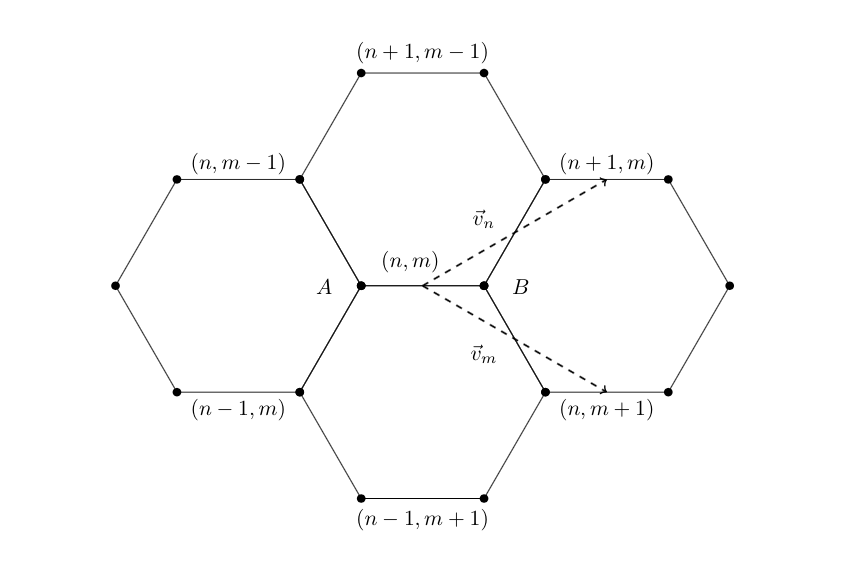
\includegraphics[width=.7\textwidth]{figures/lattice.png}
\caption{Here we draw the lattice structure of the Haldane model with cell indices labeled relative to the center cell $(n,m)$. In each cell, the 
$A$-site is the left atom and the $B$-site is the right atom. We show basis vectors $\vec{v}_n$ and $\vec{v}_m$, which allow translation to any cell in the lattice.}
\label{fig:2d Structure}%
\end{figure}

\begin{figure}
\centering
\subfloat{{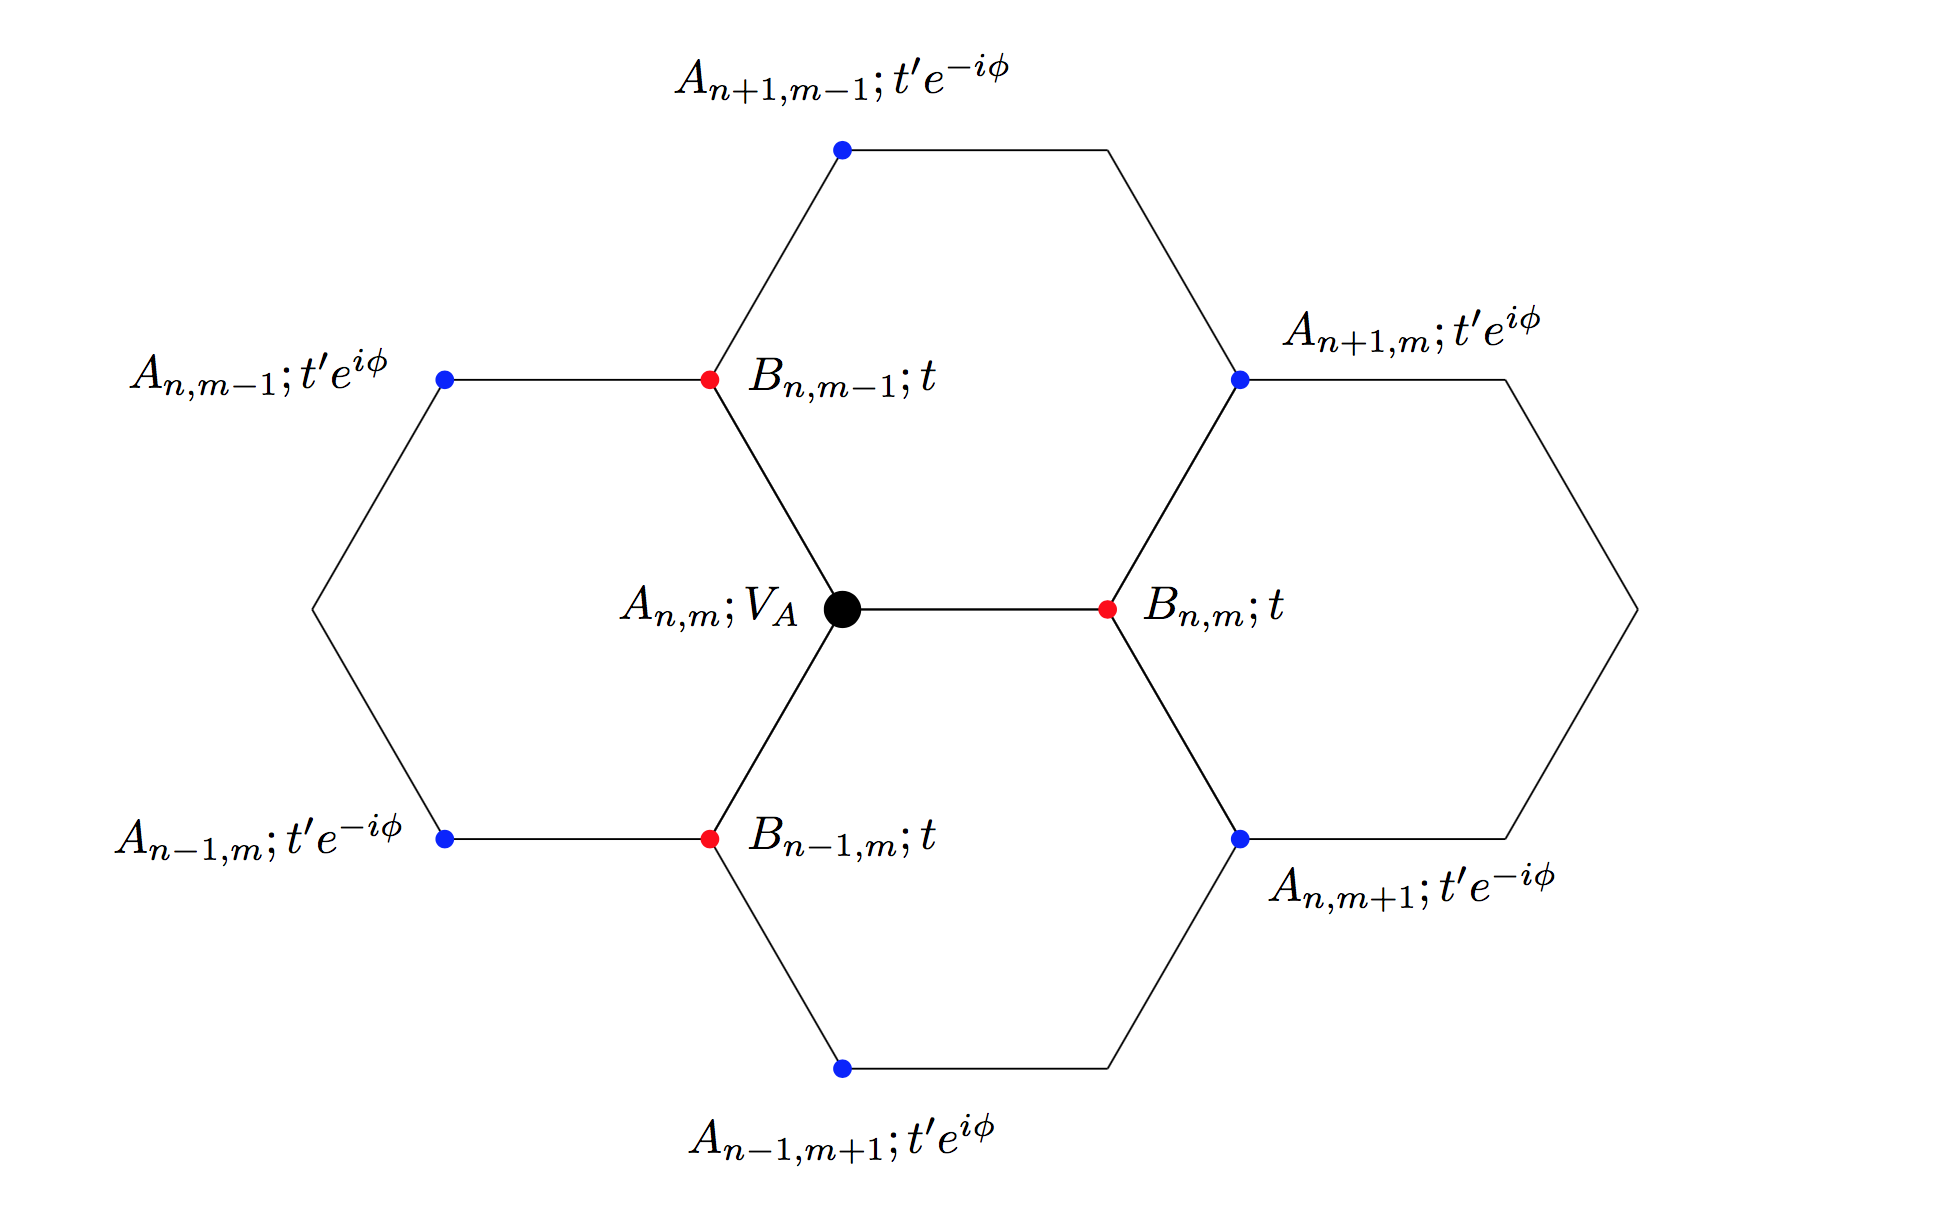
\includegraphics[width=.9\linewidth]{figures/haldane_strengths_A.png} }}%

\subfloat{{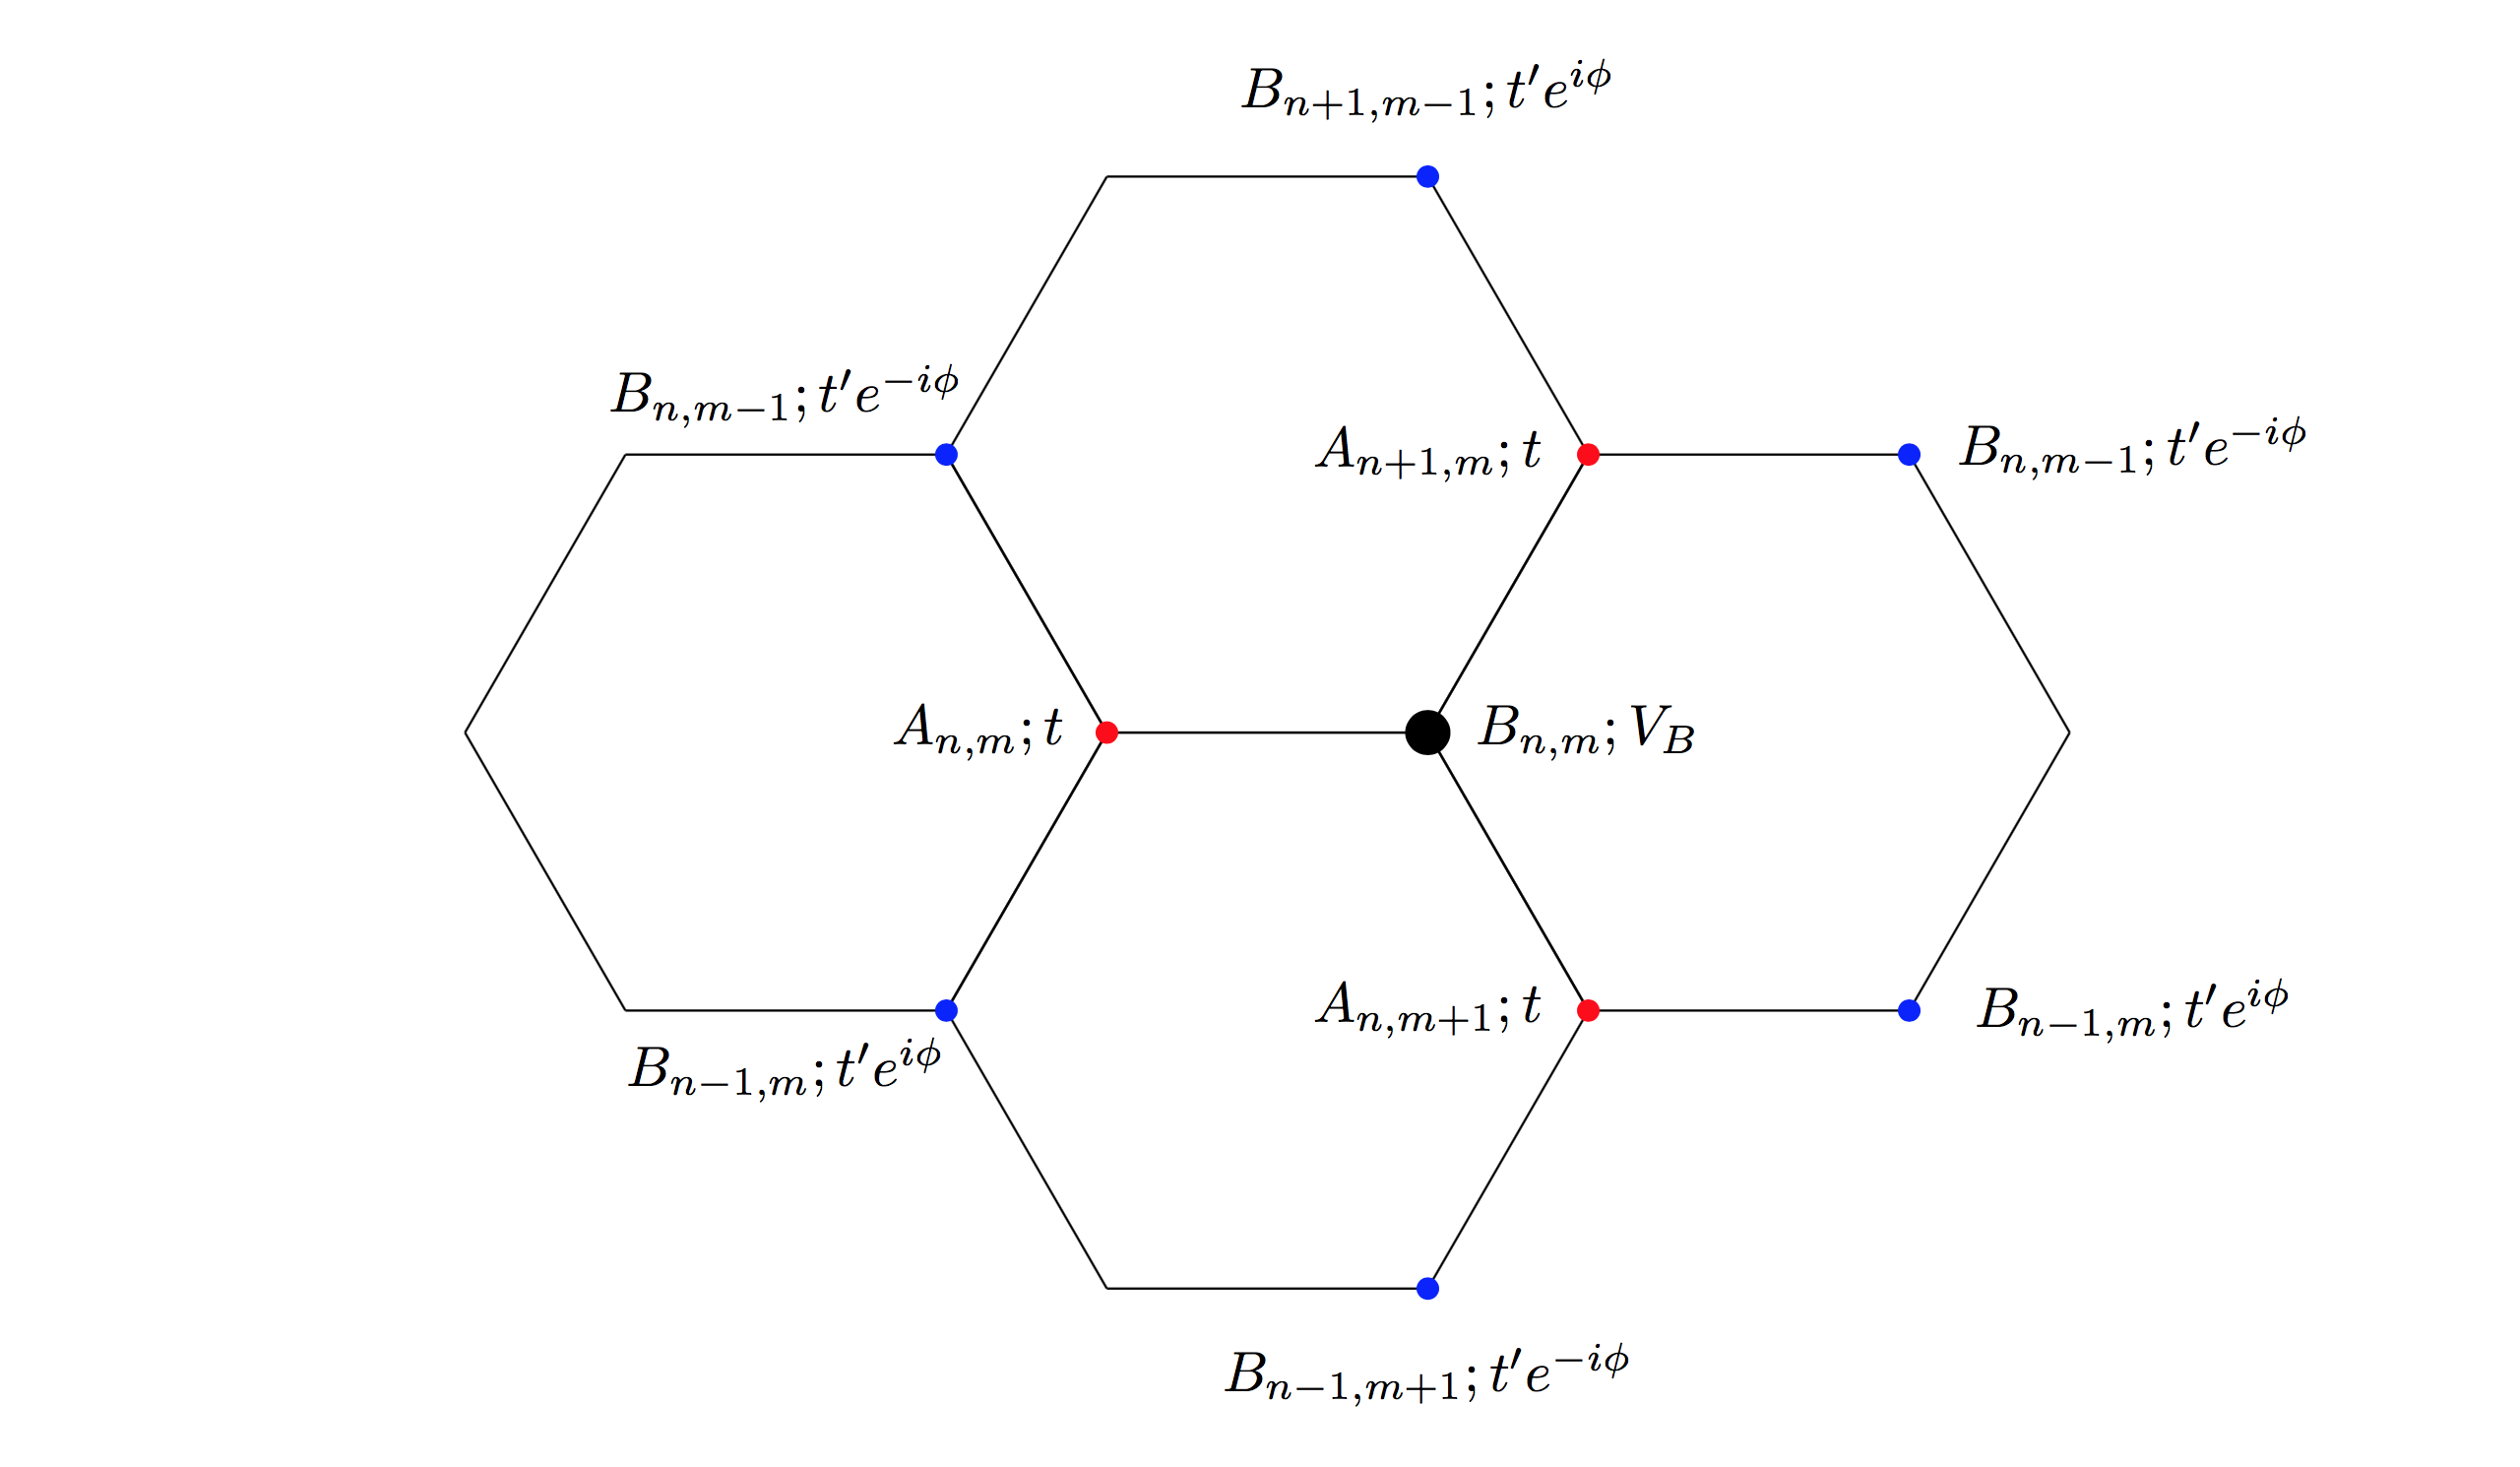
\includegraphics[width=.9\linewidth]{figures/haldane_strengths_B.png} }}%

\caption{Haldane Model Hopping Amplitudes for A and B Sites}%
\label{fig:hopping amplitudes}%
\end{figure}

We depict the hopping amplitudes of the Haldane Model in figure \ref{fig:hopping amplitudes}. We label on-site potentials $V_A, V_B \in \mathbb{R}$, nearest-neighbor hopping amplitudes $t\in \mathbb{R}$, and complex next-nearest neighbor hopping amplitude $t'e^{\pm i\phi}$, with $t'\in\mathbb{R}$ and $\phi\in[0,2\pi]$. We denote the Hamiltonian of the system $H$. We denote states of the system as vectors $\psi$ with entries $\psi_{m,n} \in \mathbb{C}^2$ where the first component of $\psi_{m,n}$ represents the part of the state at the $A$ site of the $m$, $n$th cell and the second represents the part at the $B$ site of the $m$, $n$th cell.

\subsection{Clifford Index on Lattice}
Defining the Clifford index on this system so that it is equivalent to the Chern number requires us to first define two position matrices $X$ and $Y$ as follows.

%We consider a quantum mechanical system with Hamiltonian $H$. Let $\Psi$ be a state in two dimensions with entries $\Psi_{m,n}$, where $m$ describes location with respect to one dimension (whether that be an $x$-coordinate in $\mathbb{R}^2$ or a cell index along an edge) and where $n$ describes location with respect to the other dimension.
Define $X$ and $Y$ to be the operators that act on a state $\Psi$ in the following way:
\begin{equation}\label{eq:xy}
(X \Psi)_{m,n} = m\Psi_{m,n}, \quad (Y \Psi)_{m,n} = n\Psi_{m,n}.
\end{equation}
Eigenstates of these operators are localized in their corresponding dimensions: if $\Psi$ is an eigenstate of $X$ with eigenvalue $\lambda$, then
\begin{equation}
(X \Psi)_{m,n} = m\Psi_{m,n} = \lambda\Psi_{m,n}
\end{equation}
which implies that
\begin{equation}
\Psi_{m,n} = 0 \text{ for } m \neq \lambda.
\end{equation}
Thus $\Psi$ is 0 everywhere except when $m = \lambda$, and approximate eigenstates of $X$ with eigenvalue $\lambda$ will be localized near the points where $m = \lambda$.
The same applies for $Y$.

We seek approximate simultaneous eigenstates of the three operators $X$, $Y$, and $H$. As we saw in Section \ref{sec:Cliff_ind}, such states can be computed by computing the Clifford spectrum.

%Therefore, when looking for localized eigenstates of a system whose Hamiltonian is $H$, our aim is to find simultaneous eigenstates of all three operators $H$, $X$, and $Y$.\\
%This is not always possible, however.
%Suppose $A_1,...,A_n$ are Hermitian matrices that all commute with each other.
%Then, they can be simultaneously diagonalized, i.e. $U^* A_i U$ is diagonal for all $i \in \{1,...,n\}$ for some unitary matrix $U$.
%So if $H$, $X$, and $Y$ commute, we can find simultaneous eigenstates of them.
%Now, suppose $A_1,...,A_n$ do not all commute, but their commutators are bounded:
%$$[A_i,A_j] \leq \delta \quad \forall\; i,j \in \{1,...,n\}$$
%for some $\delta$.
%If $n = 2$, there must exist some $\widetilde{A}_1, \widetilde{A}_2$ which commute and satisfy:
%$$||\widetilde{A}_1 - A_1||, ||\widetilde{A}_2 - A_2|| \leq \epsilon(\delta)$$
%where $\epsilon(\delta) \rightarrow 0$ as $\delta \rightarrow 0$ and where $||M||$ denotes the largest eigenvalue of $M$.\\
%But if $n = 3$, there may or may not exist $\widetilde{A}_1, \widetilde{A}_2, \widetilde{A}_3$ such that they all commute with each other and satisfy:
%$$||\widetilde{A}_i - A_i|| \leq \epsilon(\delta), \quad \i \in \{1,2,3\}.$$
%This existence holds if and only if
%$$\frac{1}{2}\; \text{sig} \begin{pmatrix}
%A_3 & A_1 + iA_2\\
%A_1 - iA_2 & - A_3
%\end{pmatrix} = 0$$
%where sig$(M)$ is the signature, or number of positive eigenvalues minus negative eigenvalues, of $M$. This is known as the Clifford Index of three matrices, denoted \text{ind}($A_1,A_2,A_3$).
%Thus, to calculate the index at a particular location, $\lambda_1,\lambda_2$ in our system near an eigenvalue $\lambda_3$ of $H$ \jm{Is this the correct motivation?} \aw{We actually don't assume we are near an eigenvalue of $H$. The theory just tells us that we can find approximate eigenvectors of $H, X, Y$ by finding eigenvectors corresponding to zero eigenvalues of the matrix $B$. The reason we look at $\lambda_3 = 0$ is because this is where we expect to see edge states.} we look at
%$$B(X-\lambda_1,Y - \lambda_2, H - \lambda_3) = \frac{1}{2}\; \text{sig}\begin{pmatrix}
%H - \lambda_3 & (X - \lambda_1) + i(Y - \lambda_2)\\
%(X - \lambda_1) - i(Y - \lambda_2) & - (H - \lambda_3)
%\end{pmatrix}.$$
%If this matrix has an eigenvalue less than a specified norm $\epsilon$, we say that the triple $(\lambda_1,\lambda_2,\lambda_3)$ is in the joint pseudo-spectrum of the given lattice.\aw{it is $(\lambda_1,\lambda_2,\lambda_3)$ that is in the joint pseudo-spectrum: the pseudo-spectrum is a generalization of the spectrum (the set of eigenvalues), and the joint pseudo-spectrum is a generalization of the joint spectrum}
%If a triple is not in the pseudo-spectrum, we then compute the Bott index using the above calculation. \aw{Hastings-Loring explains the Clifford index a little. The point is that } \\\\

%In the Haldane model specifically, we define our $X$ and $Y$ operators as follows (so that they may satisfy \eqref{eq:xy}).
%\begin{equation}
%X_{i,i} = \left\lfloor \frac{i-1}{2} \right\rfloor \;\text{mod}\;m, \quad\quad Y_{i,i} = \left\lfloor \frac{i-1}{2m} \right\rfloor
%\end{equation}
%with $X_{i,j} = Y_{i,j} = 0$ for $i \neq j$.

We compute the Clifford pseudospectrum and index on the Haldane model lattice and see that the Clifford index is equivalent to the Chern number.
We examine two parameter settings, one we call trivial and the other topological.
In the trivial setting, our parameters are:
\begin{equation}
V_a = 1, t = 1, t' = 0.
\end{equation}
In this case we see a Clifford index of 0 everywhere, which is also what we see with the Chern number.
In the topological setting, our parameters are:
\begin{equation}
V_a = 0, t = 1, t' = 1.
\end{equation}
The Clifford Index in this case also agrees with the Chern number, where interior sites have index 1 and exterior sites have index 0.
This is shown in Figure \ref{fig:haldane_index}.
\begin{figure}
\centering
\subfloat{{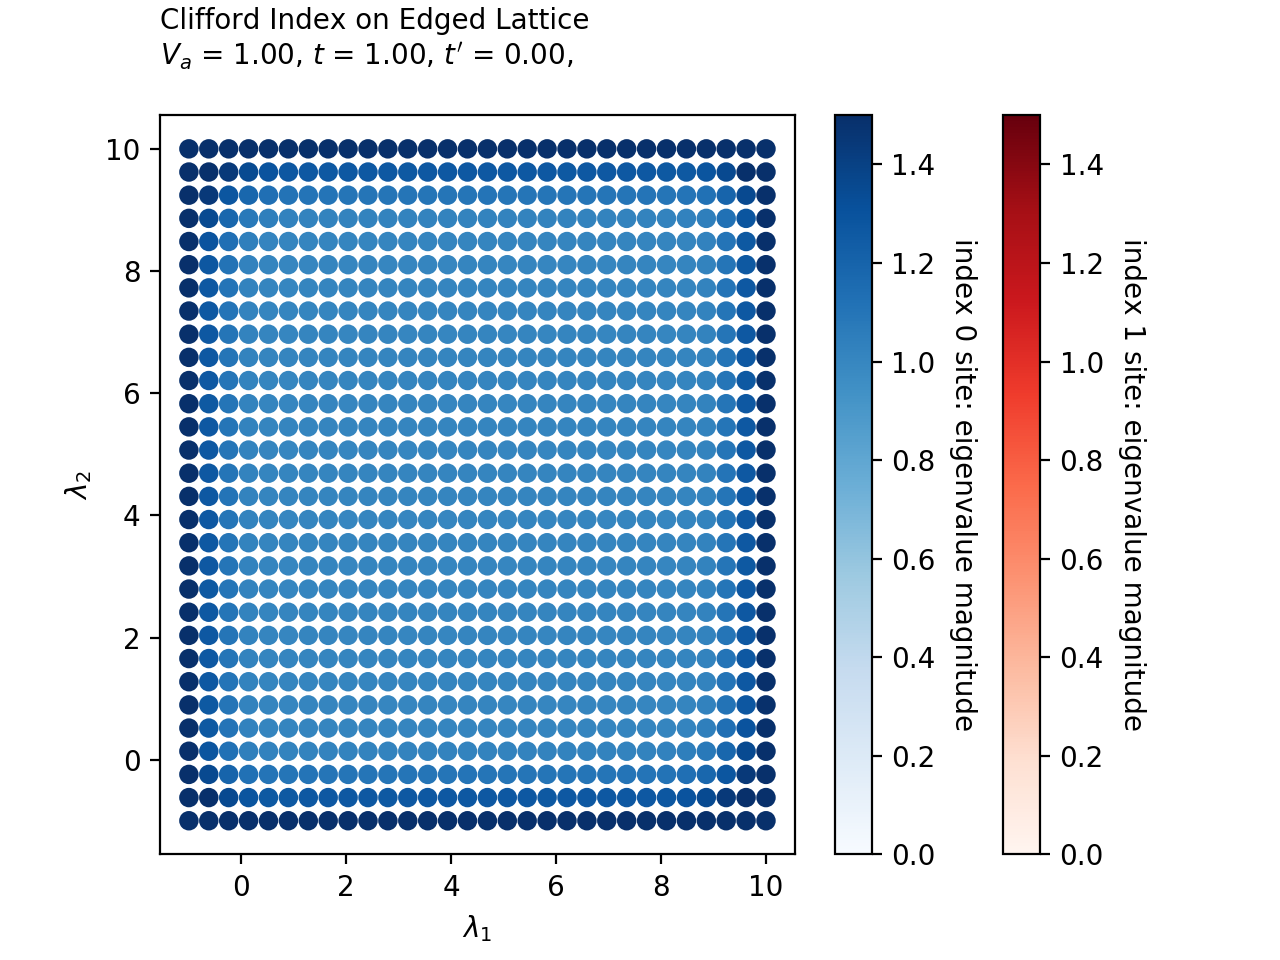
\includegraphics[width =.45\linewidth]{figures/edged_triv} }}%
\subfloat{{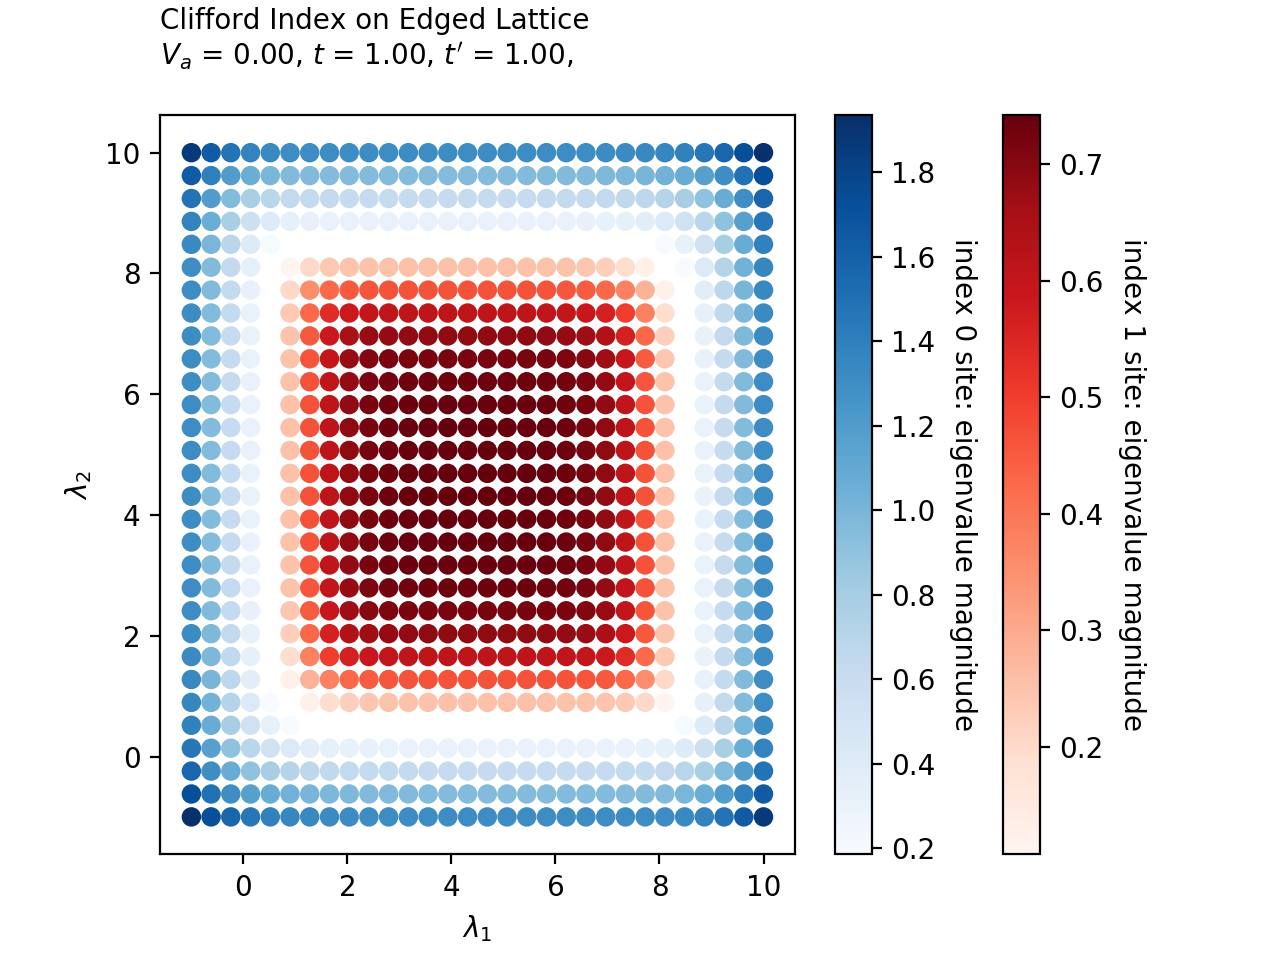
\includegraphics[width =.45\linewidth]{figures/edged_top} }}%
\caption{Clifford Index on Trivial and Topological Haldane Lattices: the left is a trivial lattice, and the right is a topological lattice, in that the parameters $V_a, t,$ and $t'$, when put on a periodic lattice, yield a Chern number of 0 and 1 respectively.
Each point in these figures represents a $(\lambda_1,\lambda_2,\lambda_3)$ triple with $\lambda_3 = 0$.
If a point is not plotted, then it is in the pseudo-spectrum, i.e. $B(X - \lambda_1, Y - \lambda_2, H - \lambda_3)$ has a near-zero eigenvalue.
If a site is not in the pseudo-spectrum, then it is colored red for index 1 and blue for index 0.
The intensity of the color represents the absolute value of the smallest eigenvalue of $B$.
So a more intense color means a larger spectral gap at that location in the lattice.
We see that in the topological case, the interior is a region of index 1, whereas in the trivial case, there are only points of index 0.
}%
\label{fig:haldane_index}%
\end{figure}
The advantage of the Clifford index compared to the Chern number is that the Chern number can only be defined on a periodic structure, whereas the Clifford index can be computed on non-periodic media.
We will use this advantage to study the robustness of waves on disorded media.

\subsection{Computational Efficiency in Computing the Clifford Index}

Computing the signature of $B$ can be done simply by finding all of the eigenvalues and calculating the number of positive minus the number of negative values.
However we can compute this more efficiently by exploiting a useful decomposition.
Let $B = LDL^t$, where $L$ is unit lower triangular and $D$ is block diagonal with blocks of order 1 or 2.
It is known (see \jm{BunchKaufman}) that the signature of $B$ equals the signature of $D$.
And the signature of $D$ is the number of positive $1 \times 1$ blocks minus the number of negative $1 \times 1$ blocks.
This greatly speeds up the computations of the Clifford index.

\section{Propagation of States Along Index Boundary in the Haldane Model}

Having verified numerically that the Clifford index and Chern number agree on the Haldane model lattice, we now show the significance of these indices.
Assume there are two regions of differing index in the lattice, near to each other such that there is a boundary between them.
As shown in section \ref{sec:clif_ind}, there are points on this boundary that are in the Clifford spectrum.
Thus, at such a boundary point $(\lambda_1,\lambda_2,\lambda_3)$, there exists a simultaneous approximate eigenvector of $X-\lambda_1$, $Y-\lambda_2$, and $H-\lambda_3$, i.e. an eigenstate of the Hamiltonian which is localized near $(\lambda_1,\lambda_2) \in \mathbb{R}^2$.
This eigenstate is the larger of $v$ and $w$, satisfying:
\begin{equation}
B(X-\lambda_1,Y-\lambda_2,H-\lambda_3) \begin{pmatrix}v\\w\end{pmatrix} = 0
\end{equation}
as shown by the calculation starting with \eqref{eq:B_eq}.
Note that it is the larger of $v$ and $w$ because in the previous calculation we assumed without loss of generality that $v > w$, even though this need not be the case.
 
In the previous section we looked at the edged Haldane model with topological parameters which gave it an interior region of index 1 and an exterior region of index 0.
Hence, we can find approximate eigenstates of the Hamiltonian localized along the edge of the lattice.
In Figure \ref{fig:haldane_prop}, we find such an edge state and simulate its propagation along the edge of the lattice using the Schr{\"o}dinger equation.
We see that the wave successfully propagates along this index boundary as expected.

\begin{figure}
\centering
\subfloat{{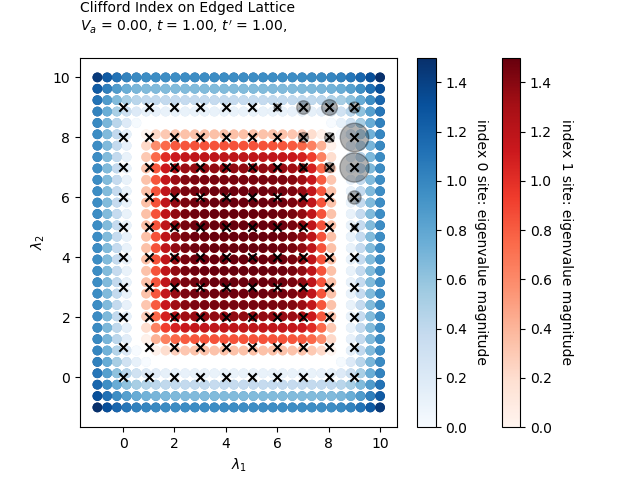
\includegraphics[width=.45\linewidth]{figures/haldane_propagation/img01.png} }}%
\subfloat{{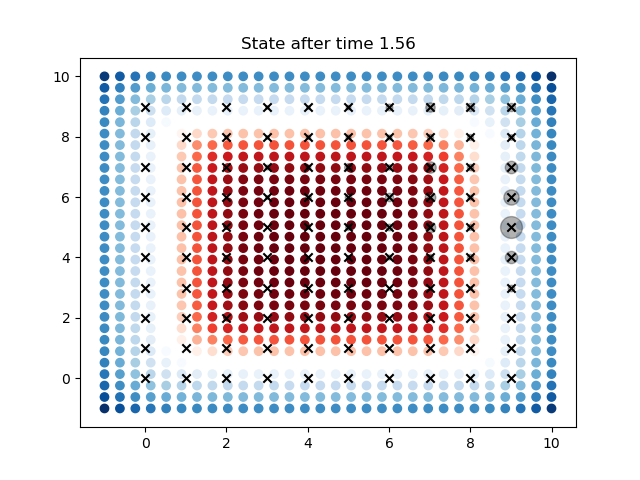
\includegraphics[width=.45\linewidth]{figures/haldane_propagation/img02.png} }}%

\subfloat{{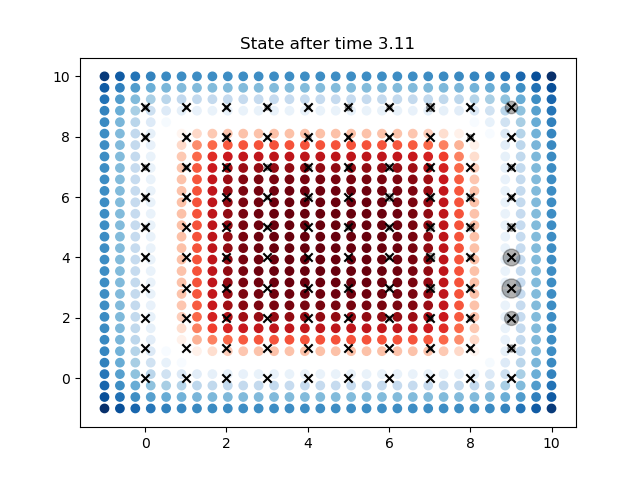
\includegraphics[width =.45\linewidth]{figures/haldane_propagation/img03.png} }}%
\subfloat{{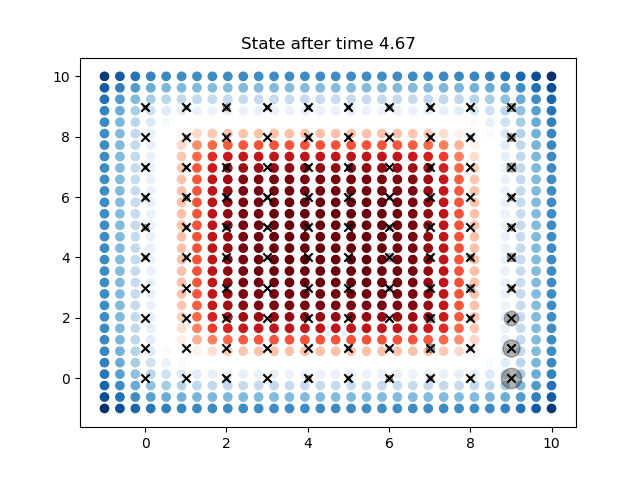
\includegraphics[width =.45\linewidth]{figures/haldane_propagation/img04.png} }}%

\subfloat{{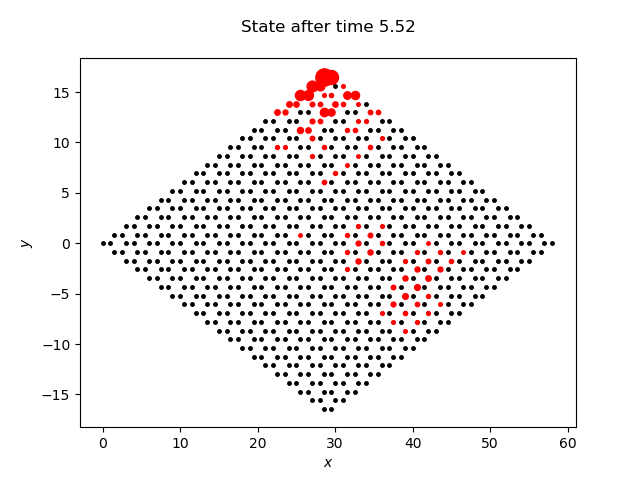
\includegraphics[width=.45\linewidth]{figures/haldane_propagation/img05.png} }}%
\subfloat{{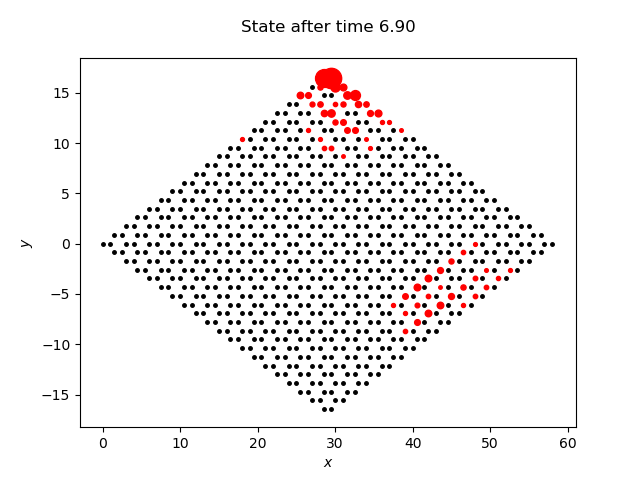
\includegraphics[width=.45\linewidth]{figures/haldane_propagation/img06.png} }}%

\subfloat{{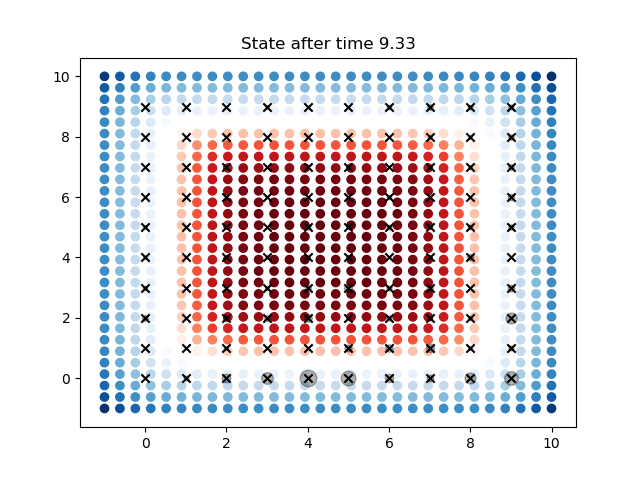
\includegraphics[width =.45\linewidth]{figures/haldane_propagation/img07.png} }}%
\subfloat{{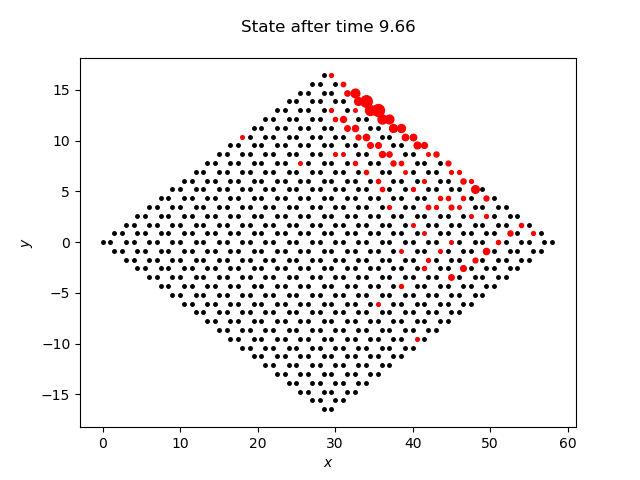
\includegraphics[width =.45\linewidth]{figures/haldane_propagation/img08.png} }}%
\caption{Propagation in Haldane Model: we find an approximate eigenstate of the Hamiltonian, localized on the edge, and simulate its propagation according to Schr{\"o}dinger's equation.
As before, points in parameter space of index 1 are red, points of index 0 are blue, and points in the pseudospectrum are not plotted.
Black crosses depict the location of the atomic sites in this model (Note that we are plotting with respect to site index rather than to coordinates in $\mathbb{R}^2$).
Gray circles represent the quantum state being propagated; the larger the circle, the greater the magnitude of the state at a given cell.
}%
\label{fig:haldane_prop}%
\end{figure}

Note that the lattice plots in Figure \ref{fig:haldane_prop} are square rather than hexagonal.
This is because we are plotting with respect to cell index rather than to coordinates in $\mathbb{R}^2$).
Also, this method of plotting condenses information in that the magnitudes of the a state's $A$ site value and $B$ site value are summed together and plotted as one cell rather than as two separate sites.

However, this does not affect the overall conclusion that, like the Chern number, the Clifford index can be used as a topological invariant in the Haldane model and is able to predict the existence and propagation of edge states.

\section{\texorpdfstring{$p_x + ip_y$}{px + ipy} Model} 
Having shown that the Clifford index is equivalent to the Chern number as a topological index on periodic media, which predicts the existence and propagation of edge states, we now see if the same holds true for disordered media, where the Chern number is not defined.
It is unclear how to generalize the Haldane model to disordered media, specifically because the hopping amplitudes when neighbors and next-nearest neighbors are no longer defined.
So we turn to a new model, the $p_x + ip_y$ model.

To construct this model, first generate a network of $N$ nodes (to be more consistent with physics we henceforth refer to nodes as sites) connected by edges. Define a Hilbert space $\mathcal{H}$ by associating to each site a copy of $\mathbb{C}^2$. The dimension of this space is clearly $2 N$. We denote vectors in $\mathcal{H}$ by:
\begin{equation}
	\psi = \left( \psi_1, \psi_2, ... \psi_N \right)^\top
\end{equation}
where each $\psi_j \in \mathbb{C}^2$:
\begin{equation}
	\psi_j = \left( \psi_j^A , \psi_j^B \right)^\top.
\end{equation}
We define a Hamiltonian acting on the $j$th site of the network by:
\begin{equation}
	( H \psi )_j = H_{jj} \psi_j + \sum_{ k \text{ nearest neighbors of } j } H_{jk} \psi_k,
\end{equation}
where $H_{jj}$ and $H_{jk}$ are $2 \times 2$ matrices defined by:
\begin{equation}
	H_{jj} = - \mu \sigma_z,
\end{equation}
\begin{equation}
	H_{jk} = - t \sigma_z - \frac{ i }{ 2 } \Delta \sigma_x \cos( \alpha_{jk} ) - \frac{ i }{ 2 } \Delta \sigma_y \sin( \alpha_{jk} ).
\end{equation}
Here, $\mu, t, \Delta$ are real parameters,
\begin{equation}
	\sigma_x = \begin{pmatrix} 0 & 1 \\ 1 & 0 \end{pmatrix}, \quad \sigma_y = \begin{pmatrix} 0 & - i \\ i & 0 \end{pmatrix}, \quad \sigma_z = \begin{pmatrix} 1 & 0 \\ 0 & -1 \end{pmatrix},
\end{equation}
denote the Pauli matrices, and $\alpha_{jk}$ denotes the angle of the edge between the $j$ and $k$th site relative to the $x$ axis \jm{Fulga}.%(see second slide of \verb|Loring_slides.pdf| in \verb|related_papers| directory).

Compared with the Haldane model, $\mu$ plays the role of $V^A$ (onsite potential difference between $A$ and $B$ sites, assuming $V^B = - V^A$), $t$ plays the role of $t$ (real nearest neighbor hopping), and $\Delta$ plays the role of $t'$ (strength of complex hopping). The nice thing about this model is that it involves only nearest neighbor hopping, so it is relatively easy to generalize to structures without periodicity.

In the case of a perfect square lattice the model simplifies to the following: 
\begin{equation}
\begin{split}
	(H \psi)_{mn} &= - \mu \sigma_z \psi_{mn} - t \sigma_z \left( \psi_{m+1,n} + \psi_{m-1,n} + \psi_{m,n+1} + \psi_{m,n-1} \right) \\
	&+ \frac{ i \Delta }{ 2 } \left( - \sigma_x \psi_{m+1,n} - \sigma_y \psi_{m,n+1} + \sigma_x \psi_{m-1,n} + \sigma_y \psi_{m,n-1} \right),
\end{split}
\end{equation}
where $m$ denotes the co-ordinate in the $x$ direction and $n$ denotes that in the $y$ direction. Imposing the Bloch-periodic boundary condition yields:
\begin{equation}
\begin{split}
	H(k) \psi &= \left[ - \mu \sigma_z - t \left( e^{i k_1} + e^{- i k_1} + e^{i k_2} + e^{- i k_2} \right) \sigma_z \right. \\
	&\left. + \frac{ i \Delta }{ 2 } \left( -  e^{i k_1} + e^{- i k_1} \right) \sigma_x + \frac{ i \Delta }{ 2 } \left( - e^{i k_2} + e^{- i k_2} \right) \sigma_y \right] \psi,
\end{split}
\end{equation}
\begin{equation}
	H(k) \psi = \left[ - \mu \sigma_z - 2 t \left( \cos(k_1) + \cos(k_2) \right) \sigma_z + \Delta \sin(k_1) \sigma_x + \Delta \sin(k_2) \sigma_y \right] \psi. 
\end{equation}
So:
\begin{equation}
	H(k) = \begin{pmatrix} - \mu - 2 t ( \cos k_1 + \cos k_2 ) & \Delta ( \sin k_1 - i \sin k_2 ) \\ \Delta ( \sin k_1 + i \sin k_2 ) & \mu + 2 t ( \cos k_1 + \cos k_2 ) \end{pmatrix}.
\end{equation}
Eigenvalues $E$ satisfy the characteristic equation:
\begin{equation}
	( - \mu - 2 t ( \cos k_1 + \cos k_2 ) - E )( \mu + 2 t ( \cos k_1 + \cos k_2 ) - E ) - \Delta^2 ( \sin^2 k_1 + \sin^2 k_2 ) = 0
\end{equation}
which has the solution:
\begin{equation}
	E = \pm 2 t \sqrt{ (\Delta')^2 \sin^2 k_1 + (\Delta')^2 \sin^2 k_2 + \left( \mu' + \cos k_1 + \cos k_2 \right)^2 },
\end{equation}
where:
\begin{equation}
	\Delta' := \frac{\Delta}{2 t} \quad \mu' := \frac{ \mu }{ 2 t }
\end{equation}
and now under the square root is a sum of non-negative terms. For the bands to touch (i.e. for what is under the spectral gap to vanish) it must be that:
\begin{equation}
	k_1 = m \pi \quad k_2 = n \pi
\end{equation}
for $m \in \{0,1\}$ and $n \in \{0,1\}$, and:
\begin{equation}
	\mu' + \cos m \pi + \cos n \pi = 0.
\end{equation}
This can only occur if $m = n = 1$ and $\mu' = 2$, if $m \neq n$ and $\mu' = 0$, or if $m = n = 0$ and $\mu' = - 2$.
These are the only values of $\mu'$ such that a topological transition (a change in the Chern number) can happen.
So for example, if $t = 1$, a topological transition can only occur at $\mu = \pm4$.
We check this numerically and produce Figure \ref{fig:pxipy_params}.
This is close to what we should see as there are topological transitions from zero index systems to nonzero index systems around $\mu = 4$.
These numerics allow us to choose parameters of topologically significant systems that we will study in the following section.

\begin{figure}
\centering
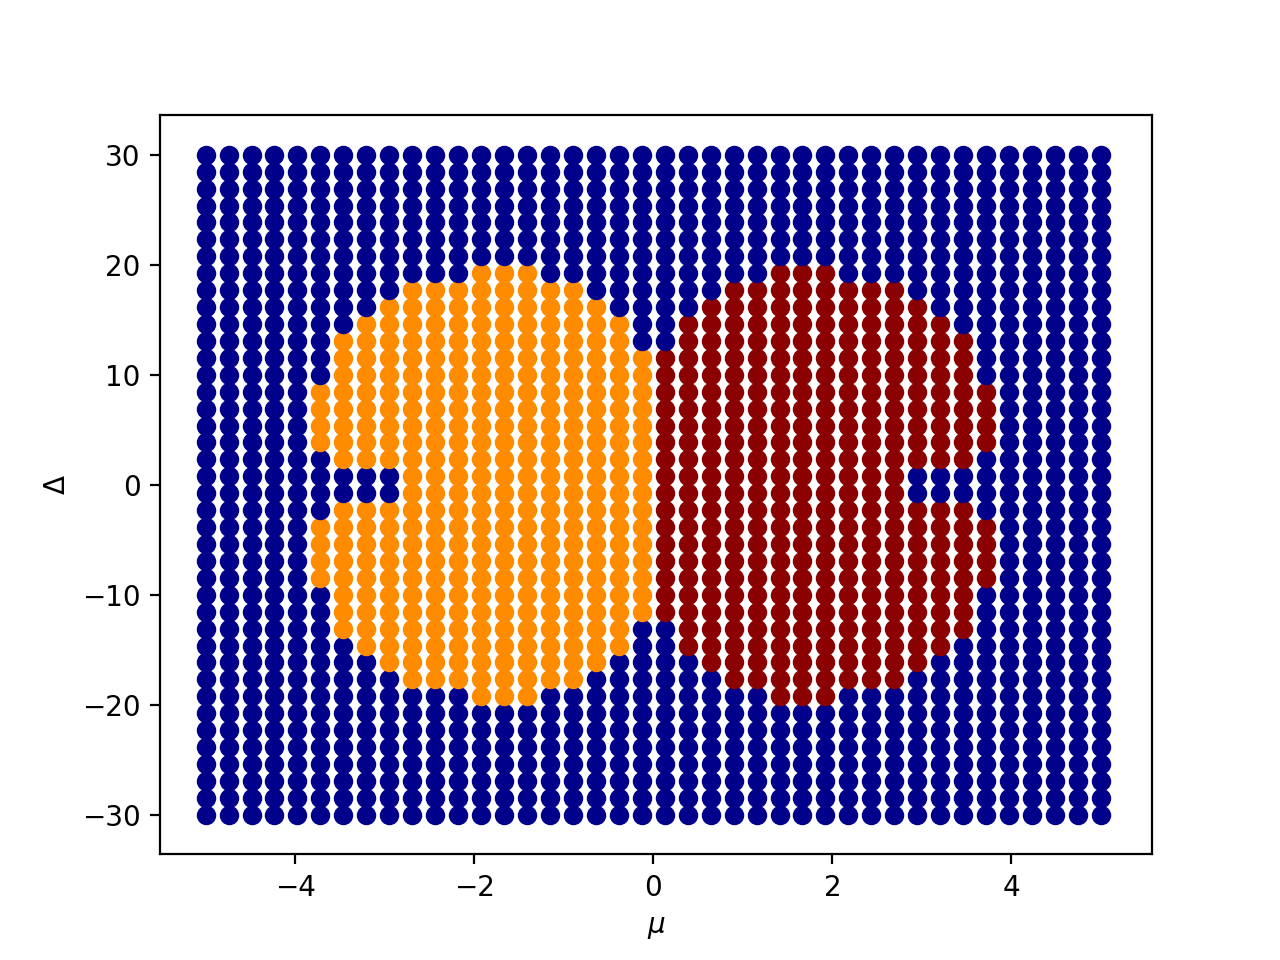
\includegraphics[width=.9\textwidth]{figures/pxipy_index_by_param.png}
\caption{Clifford Index in $p_x + ip_y$ Model with Varying Parameters: we fix $t = 1$ and let $\mu$ and $\Delta$ vary, computing the index of a point in the center of the lattice (where $\lambda_1 = \lambda_2 = 5$).
Blue represents index 0, red index 1 and orange index -1.
}
\label{fig:pxipy_params}%
\end{figure}

\section{Clifford Index in \texorpdfstring{$p_x + ip_y$}{px + ipy} Model} \label{sec:Cliff_px}
For the $p_x + ip_y$ model we compute X and Y as before in the Haldane model.
Nodes in the $p_x + ip_y$ model consist of two sites (labeled A and B) just as in the Haldane model the X and Y matrices represent this in that they are diagonal matrices of size $2mn$.
We also compute pseudo-spectrum and Clifford index as before, and get a similar result of a topological case which exhibits a transition from index 0 at the edge to 1 on the interior.
Again, this is a situation in which the system is general and not periodic so the Clifford index is useful, as we cannot use the Chern number.
The fact that we see very similar behavior in this model is very significant and supports the idea that the Clifford index is a general invariant than can be calculated regardless of periodicity or structure.

When we vary the onsite potential and atomic position, we see behavior in the Clifford index that looks less and less like the case with no disorder.
If the disorder is small, we get behavior that looks similar to the case with no disorder.
The Clifford index is 0 around the edge and 1 in the middle with pseudospectrum in between.
The only difference is that there might be some slight perturbations in where the transition occurs.
The real differences in the behavior of the system occurs when the disorder is increased (See figure \ref{fig:pxipy_index}).
When the disorder is high enough, we see that there are locations in the bulk where there exists pseudospectrum and sections where the Clifford index is 0.
This is significant because we can now study both behavior of states along the edge with perturbations and states that exist along the interface between sections of the bulk where there is differing Chern number.

\begin{figure}
\centering
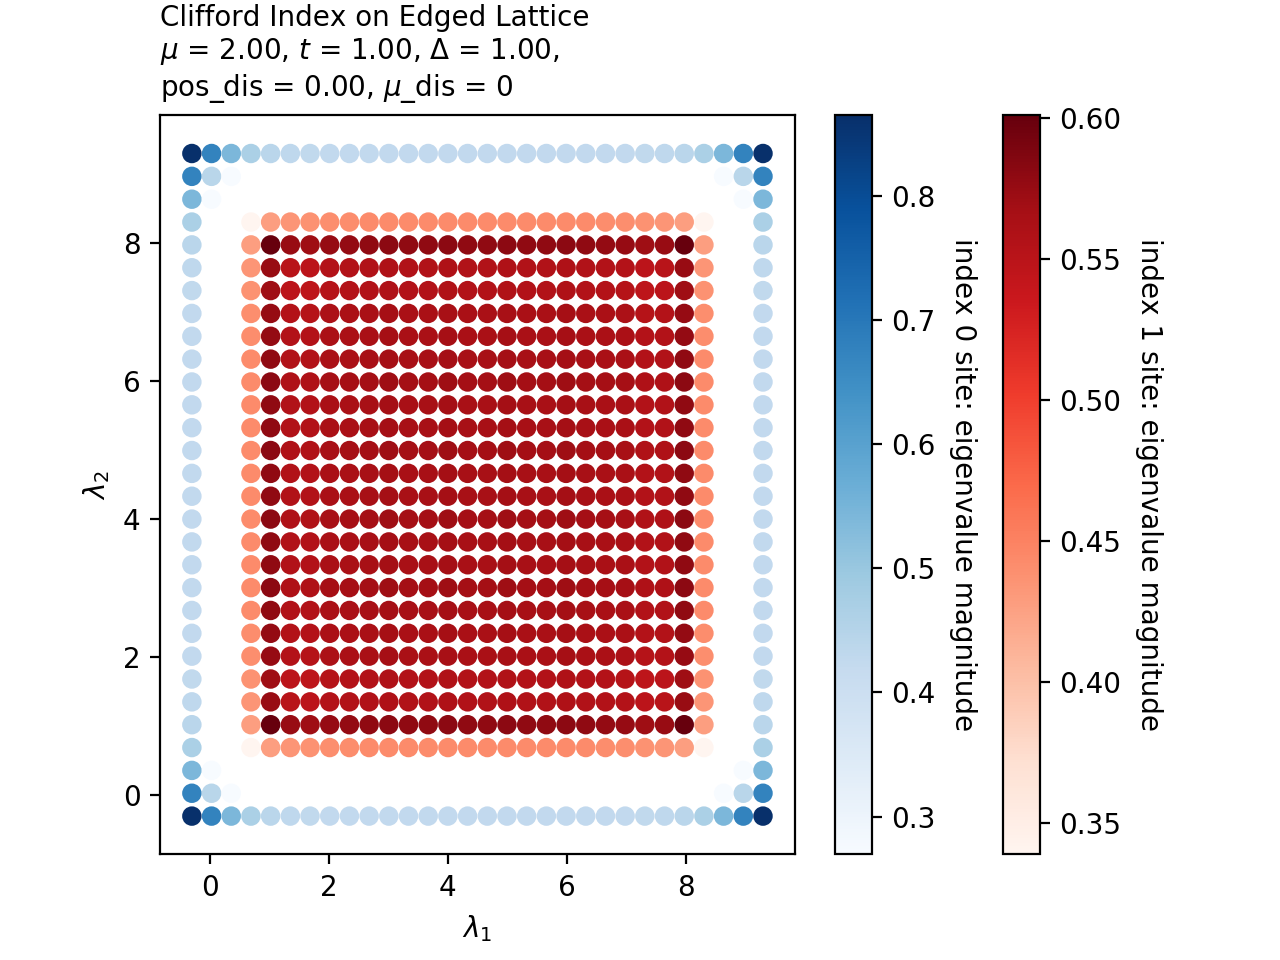
\includegraphics[width=.9\textwidth]{figures/pxipy_clifford.png}
\caption{Clifford Index in $p_x + ip_y$ Model: plotted here is the Clifford pseudospectrum and index of sites not in the pseudospectrum.
A point in parameter space with $x$-coordinate $\lambda_1$ and $y$-coordinate $\lambda_2$ is in the pseudospectrum if the matrix $B(X - \lambda_1, Y - \lambda_2, H - \lambda_3)$ \eqref{eq:B_matrix} has an eigenvalue with absolute value smaller than a given threshold.
Throughout the report, this threshold is $0.1$.
If a point is in the pseudospectrum it is not plotted and appears white on the figure.
If a point is not in the psuedospectrum, we calculate its index using \eqref{eq:index}.
Points with index 1 are plotted in red, and sites of index 0 are plotted in blue.
The intensity of the color represents the absolute value of the smallest eigenvalue of $B$.
So a more intense color means a larger spectral gap at that location in the lattice.
}
\label{fig:pxipy_index}%
\end{figure}

\begin{figure}
\centering
\subfloat{{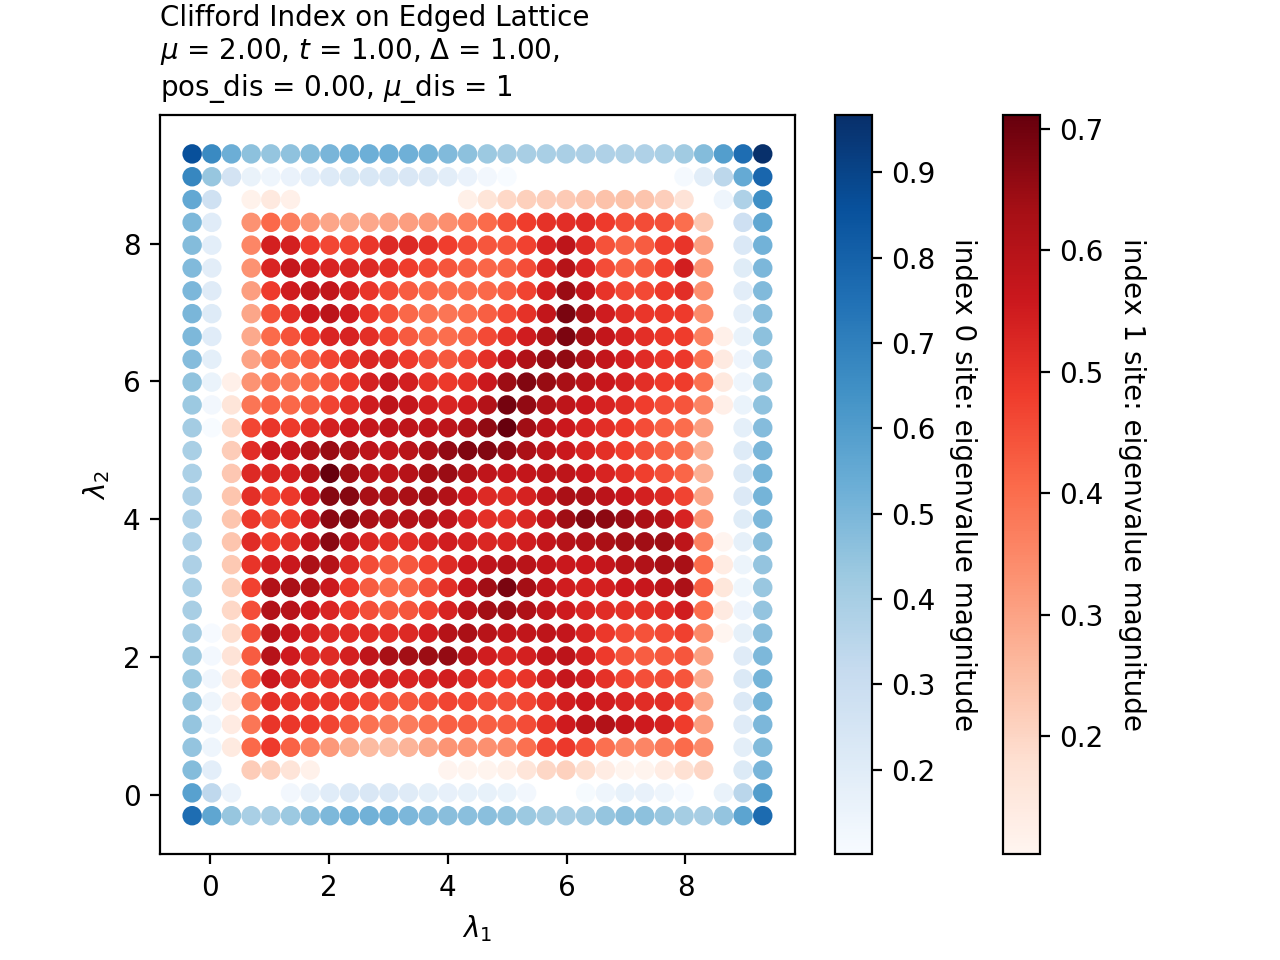
\includegraphics[width=.45\linewidth]{figures/mu_dis_index/img01.png} }}%
\subfloat{{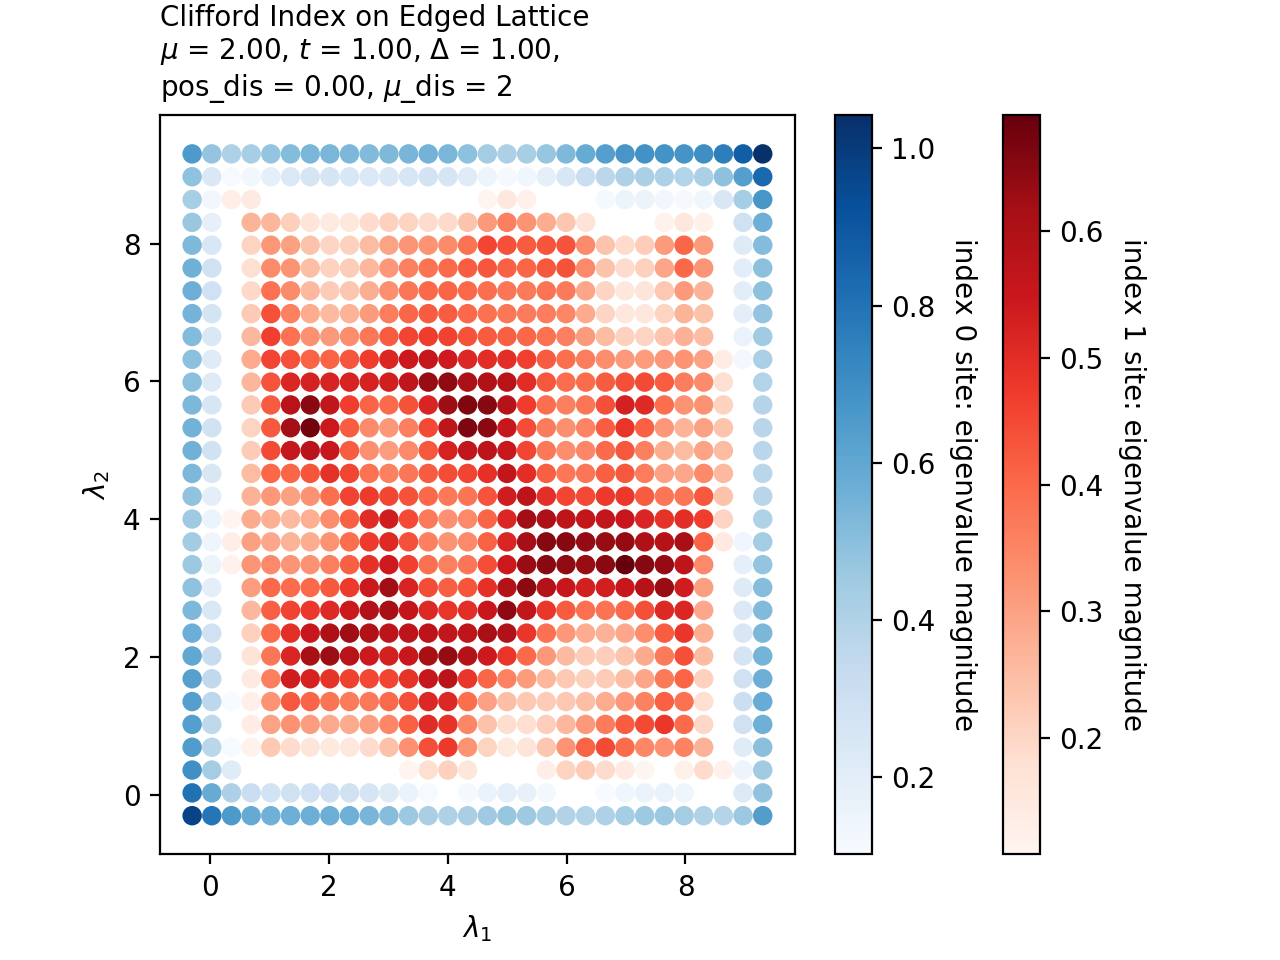
\includegraphics[width=.45\linewidth]{figures/mu_dis_index/img02.png} }}%

\subfloat{{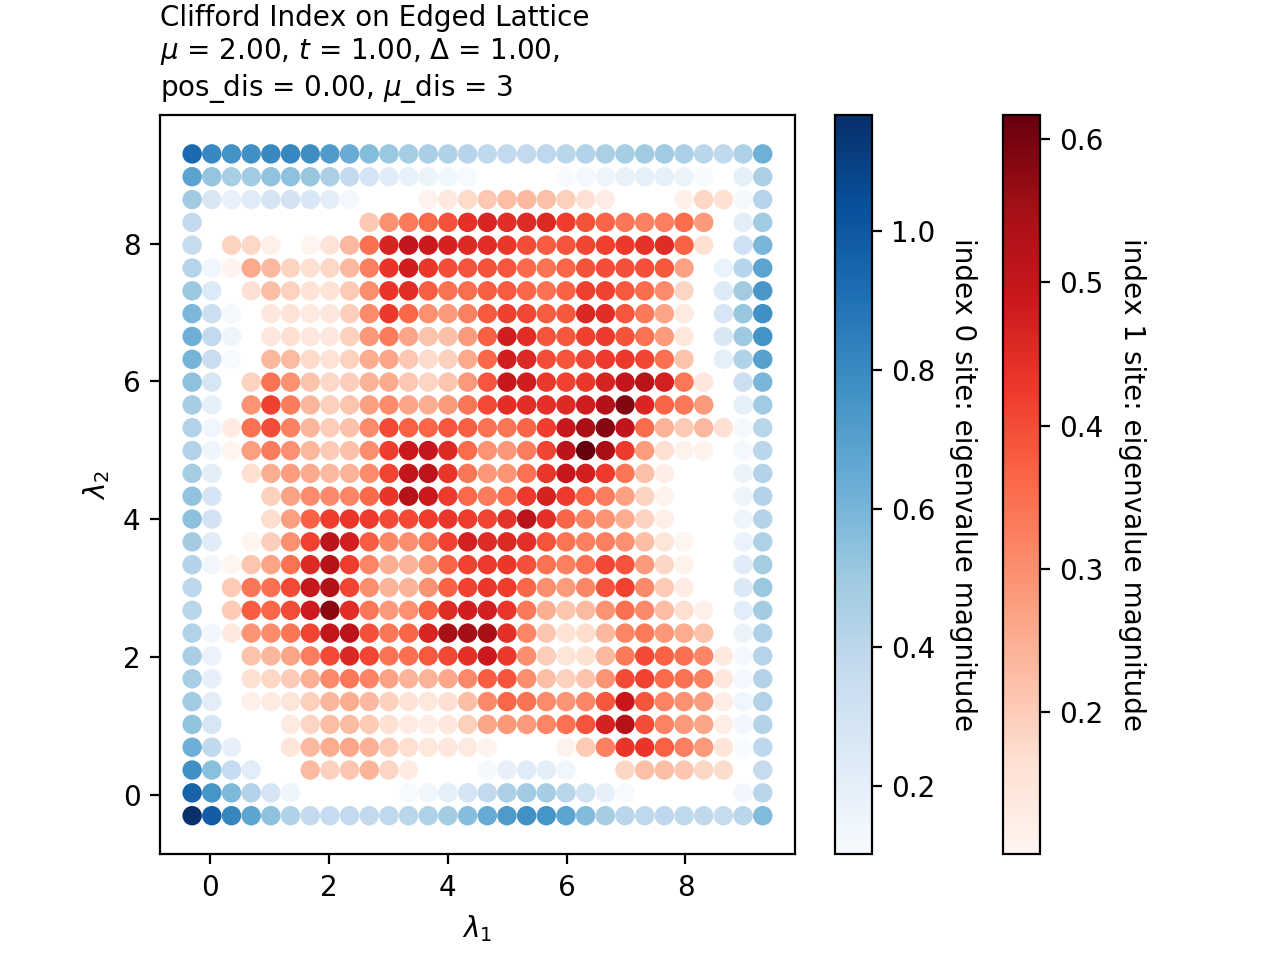
\includegraphics[width =.45\linewidth]{figures/mu_dis_index/img03.png} }}%
\subfloat{{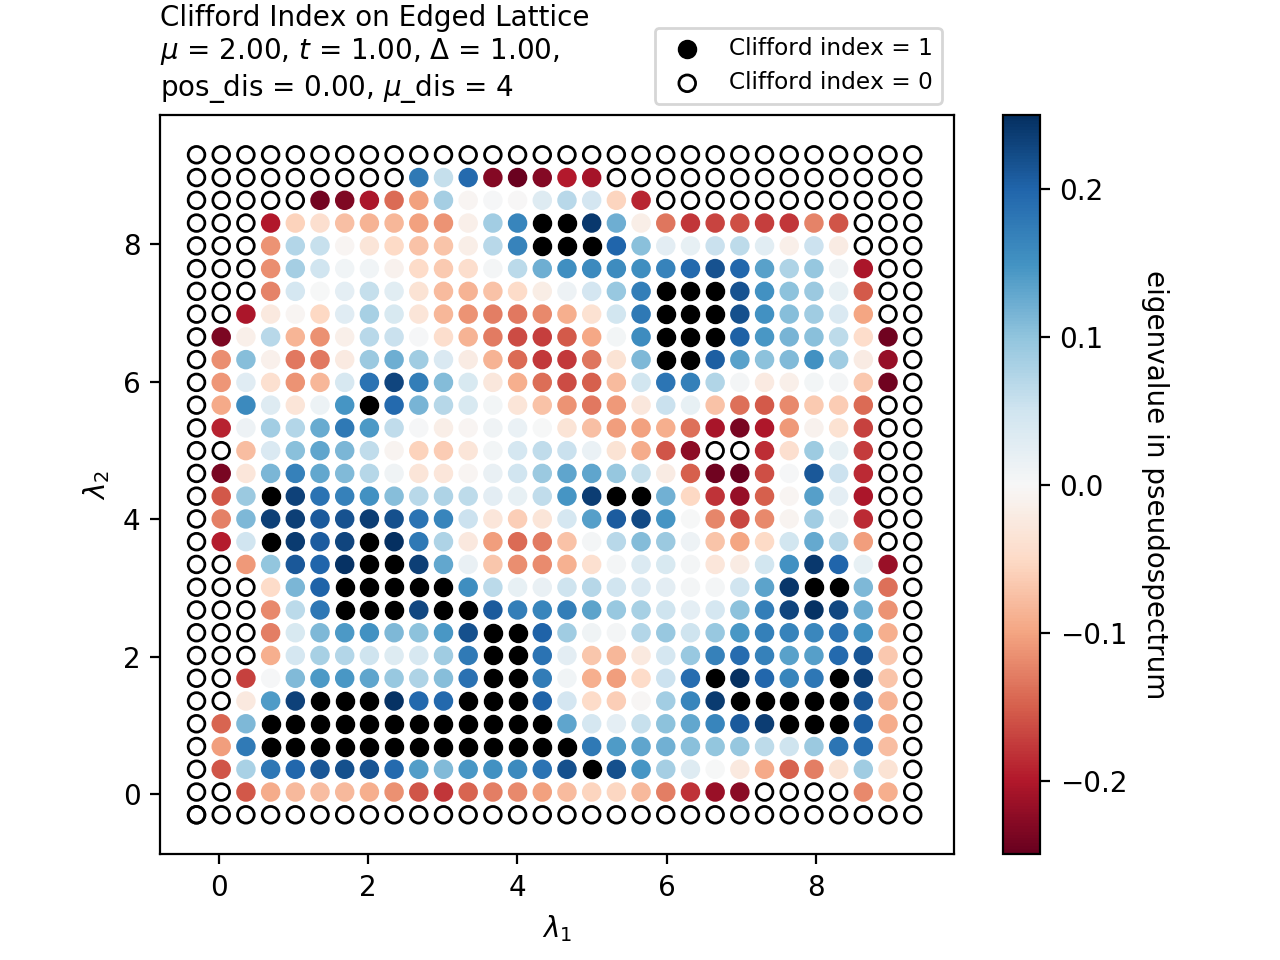
\includegraphics[width =.45\linewidth]{figures/mu_dis_index/img04.png} }}%

\caption{Clifford Index in $p_x + ip_y$ Model with Onsite Disorder: we plot the pseudospectrum and index of lattice points with varying degrees of onsite disorder.
The potential energy of each site on the lattice is chosen randomly from a uniform distribution centered at $\mu$ with the length of the interval equal to a disorder parameter: 1, 2, 3, and 4 in these plots.
So going from left to right, top to bottom, $\mu$ was chosen uniformly on $[1.5,2.5],\; [1,3],\;[0.5,3.5],$ and $[0,4]$, respectively.
Again, white represents points in the pseudospectrum, red represents points of index 1, and blue represents points of index 0.
}%
\label{fig:mu_dis_index}%
\end{figure}

\section{Propagation in \texorpdfstring{$p_x + ip_y$}{px + ipy} Model}

We will now discuss the propagation of states along interfaces in the $p_x + ip_y$ model.
When there exists no disorder, we see propagation of states localized at the edge along the interface between the areas of zero and nonzero Clifford index (See Figure \ref{fig:pxipy_prop}).
The state becomes more dispersed as time increases, but remains localized along the interface of the structure. 
When we increase disorder, both in position and in onsite potential, we see similar behavior of states localized around the edge (See Figures \ref{fig:pos_dis_prop} and \ref{fig:mu_dis_edge_prop}).
The state propagates in the same way around the edge of the lattice, remaining on the interface between zero and nonzero Clifford index.
The state disperses faster than the case in which there is no disorder, but the fact that the state still propagates around the edge suggests that even with disorder, the propagation of the edge state is still protected.
When we attempted to see propagation of states around interfaces in the bulk of the medium, we saw that they dispersed very quickly throughout the medium, so it appears this propagation is not protected (See Figure \ref{fig:mu_dis_interior_prop}).
We believe that this is because here there is not as quick a change in the Clifford index, so the interface is not as well-defined, but more research is required to determine exactly why we fail to see this behavior.


\begin{figure}
\centering
\subfloat{{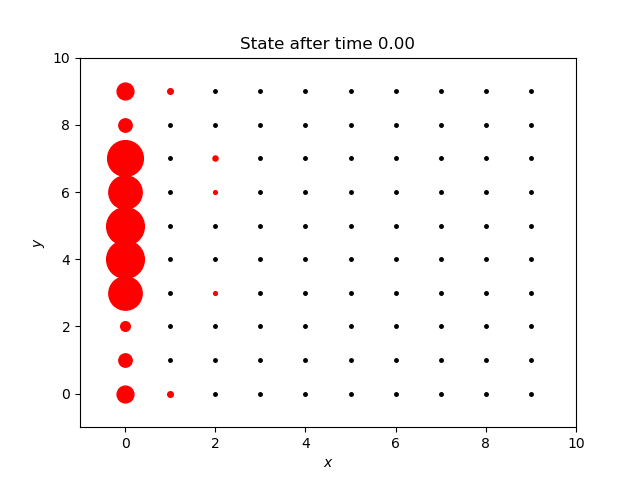
\includegraphics[width=.45\linewidth]{figures/pxipy_prop/img01.png} }}%
\subfloat{{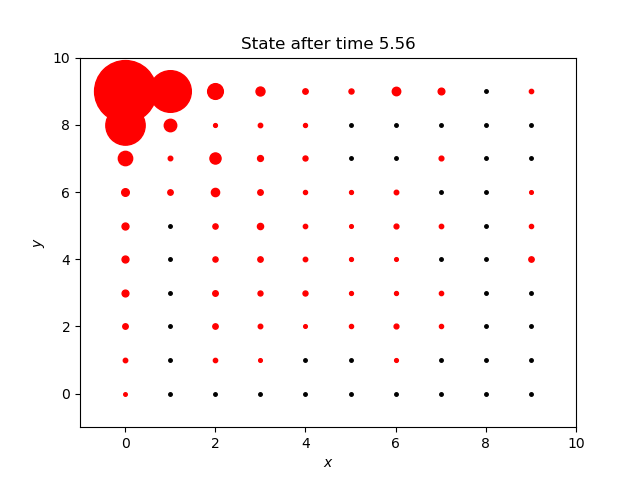
\includegraphics[width =.45\linewidth]{figures/pxipy_prop/img02.png} }}%

\subfloat{{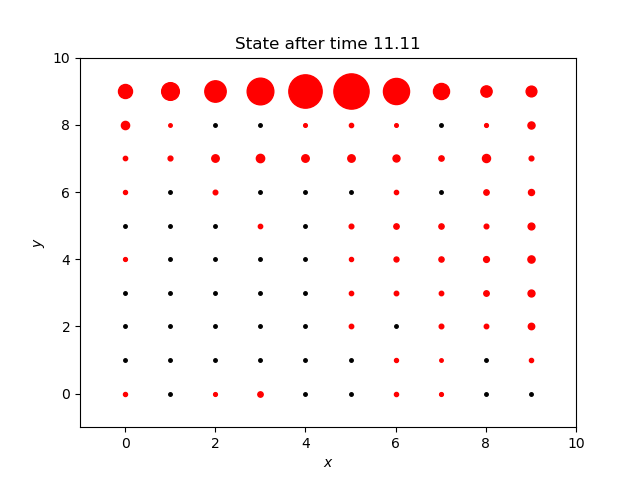
\includegraphics[width =.45\linewidth]{figures/pxipy_prop/img03.png} }}%
\subfloat{{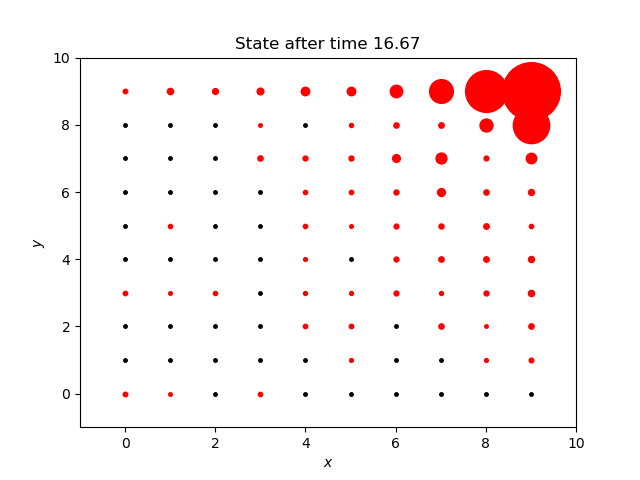
\includegraphics[width=.45\linewidth]{figures/pxipy_prop/img04.png} }}%

\subfloat{{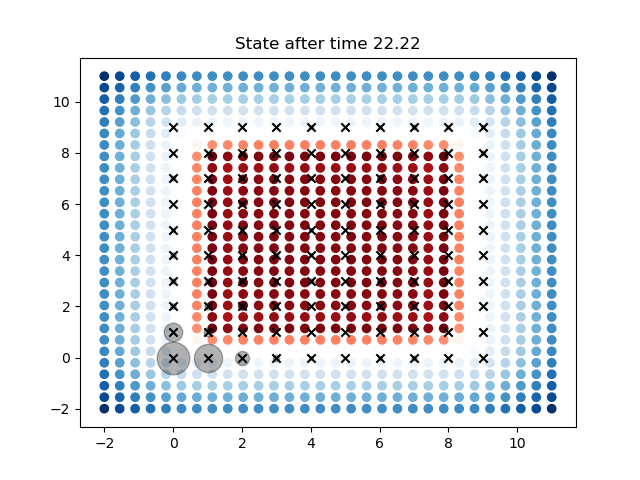
\includegraphics[width=.45\linewidth]{figures/pxipy_prop/img05.png} }}%
\subfloat{{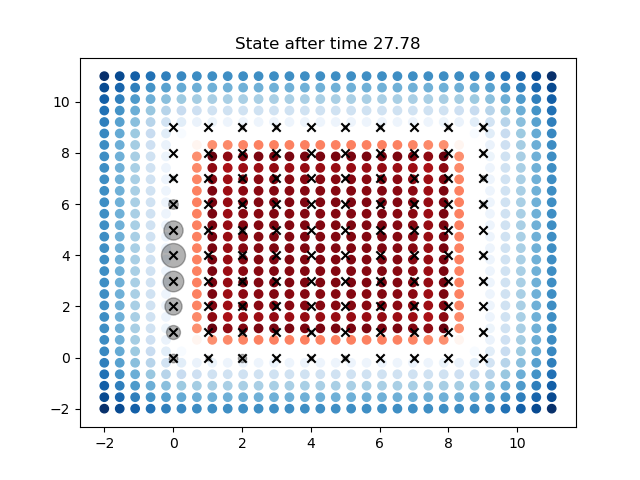
\includegraphics[width =.45\linewidth]{figures/pxipy_prop/img06.png} }}%

\subfloat{{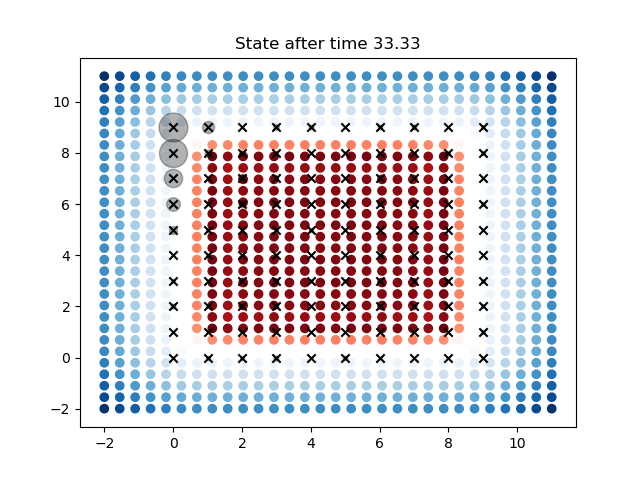
\includegraphics[width =.45\linewidth]{figures/pxipy_prop/img07.png} }}%
\subfloat{{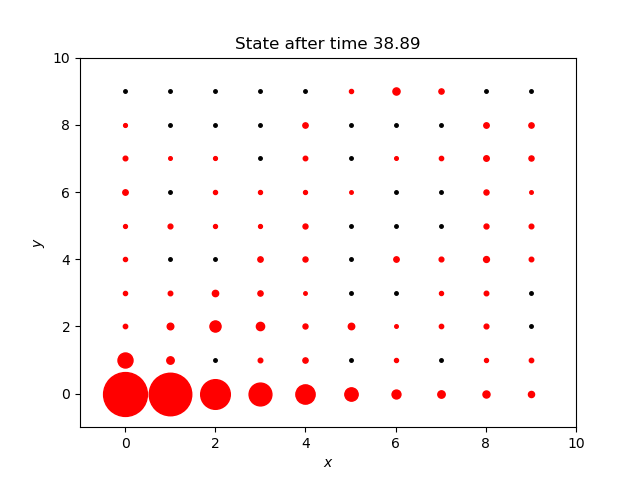
\includegraphics[width =.45\linewidth]{figures/pxipy_prop/img08.png} }}%
\caption{Propagation in $p_x + ip_y$ Model: we localize the above eigenstate along one edge of the lattice and simulate its propagation according to Schr{\"o}dinger's equation.
As before, the state is plotted in gray and $\mu = 2,\; t = \Delta = 1$.
We see the state propagate around the edge, and gradually become more dispersed as time increases.
We attribute this propagation to the fact that the edge is a boundary between a region of index 1 and a region of index 0.
}%
\label{fig:pxipy_prop}%
\end{figure}

\begin{figure}
\centering
\subfloat{{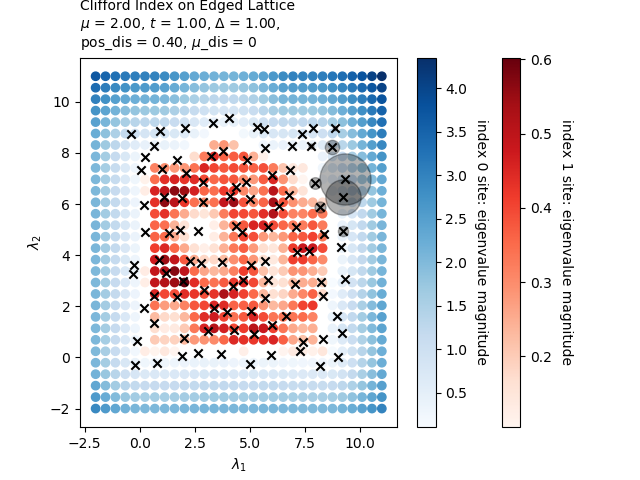
\includegraphics[width=.45\linewidth]{figures/pxipy_posdis/img01.png} }}%
\subfloat{{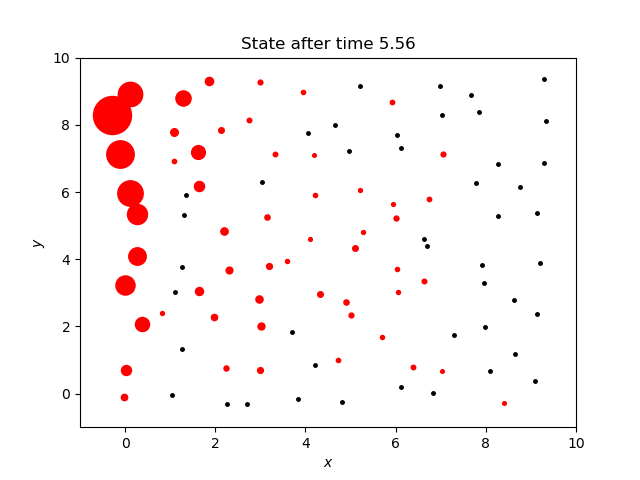
\includegraphics[width =.45\linewidth]{figures/pxipy_posdis/img02.png} }}%

\subfloat{{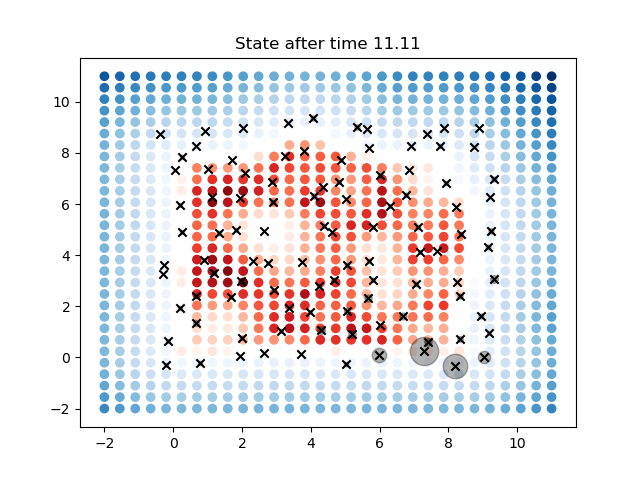
\includegraphics[width =.45\linewidth]{figures/pxipy_posdis/img03.png} }}%
\subfloat{{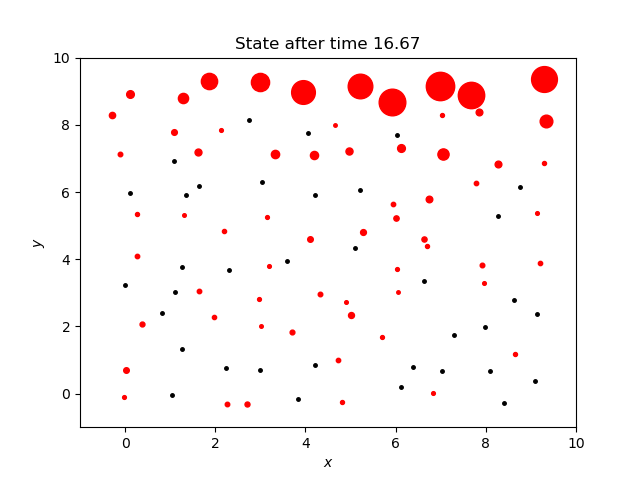
\includegraphics[width=.45\linewidth]{figures/pxipy_posdis/img04.png} }}%

\subfloat{{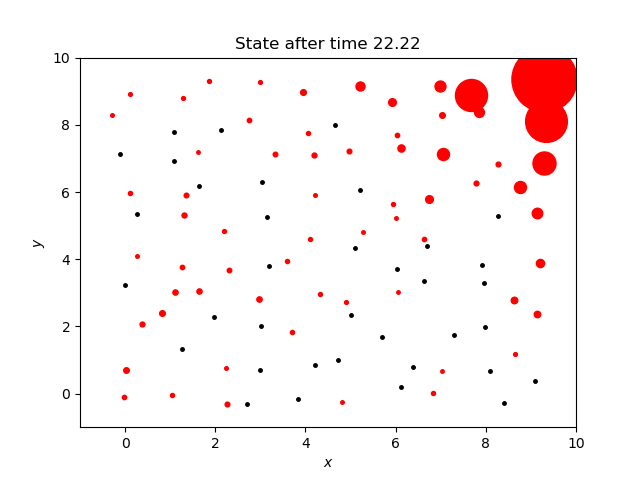
\includegraphics[width=.45\linewidth]{figures/pxipy_posdis/img05.png} }}%
\subfloat{{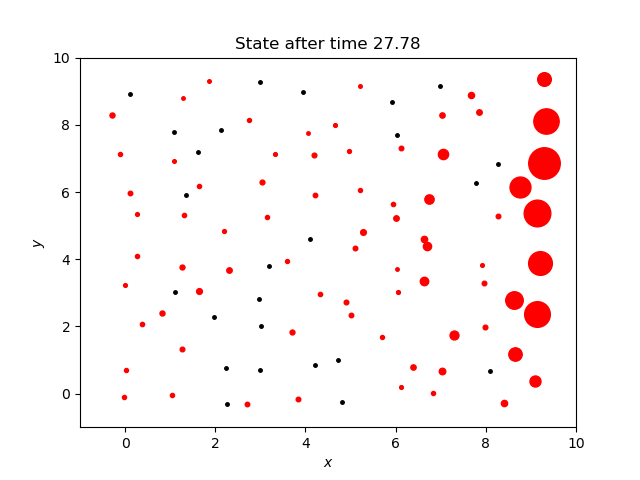
\includegraphics[width =.45\linewidth]{figures/pxipy_posdis/img06.png} }}%

\subfloat{{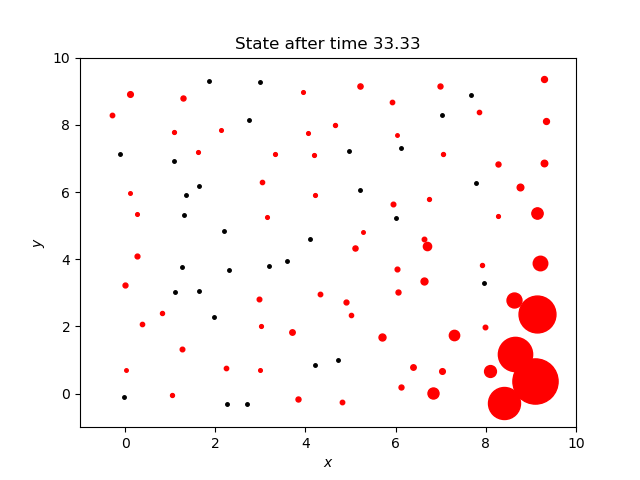
\includegraphics[width =.45\linewidth]{figures/pxipy_posdis/img07.png} }}%
\subfloat{{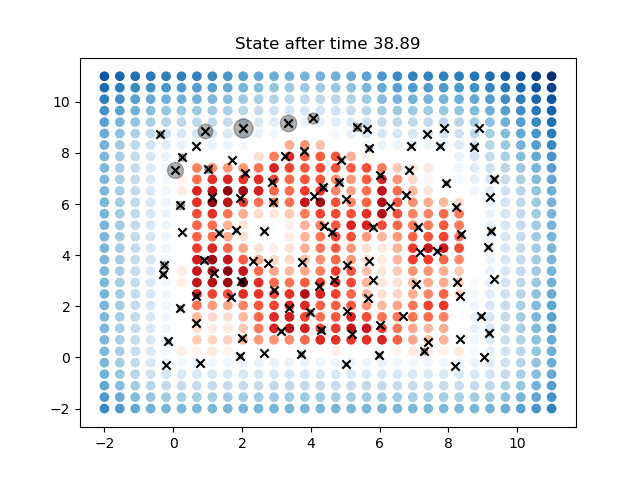
\includegraphics[width =.45\linewidth]{figures/pxipy_posdis/img08.png} }}%
\caption{Propagation in $p_x + ip_y$ Model with Position Disorder: with parameters as in Figure \ref{fig:pxipy_prop}, we now add position disorder to the lattice, i.e. we let the $x$ and $y$ coordinates of each site vary uniformly on an interval centered at its original coordinate in the lattice.
In this case, sites can deviate up to $0.4$ from its original position in either the $x$ or $y$ direction, as shown by the placement of the black x's on the plot.
We initialize a state on the edge and see continued propagation along the boundary as in the case with no disorder, however the state disperses sooner than in the case with no disorder.
}%
\label{fig:pos_dis_prop}%
\end{figure}

\begin{figure}
\centering
\subfloat{{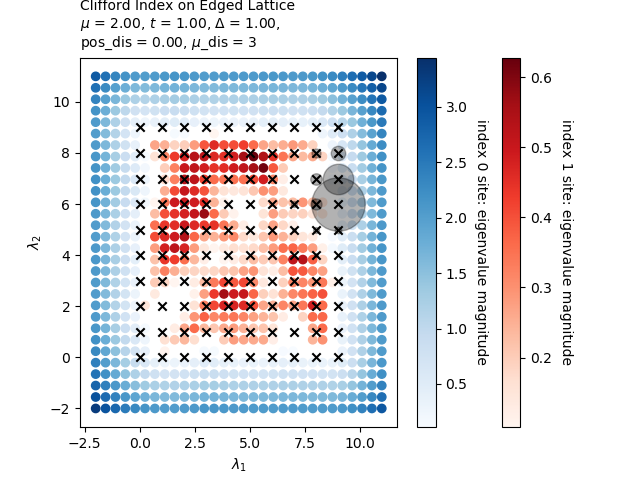
\includegraphics[width=.45\linewidth]{figures/mu_dis_edge/img01.png} }}%
\subfloat{{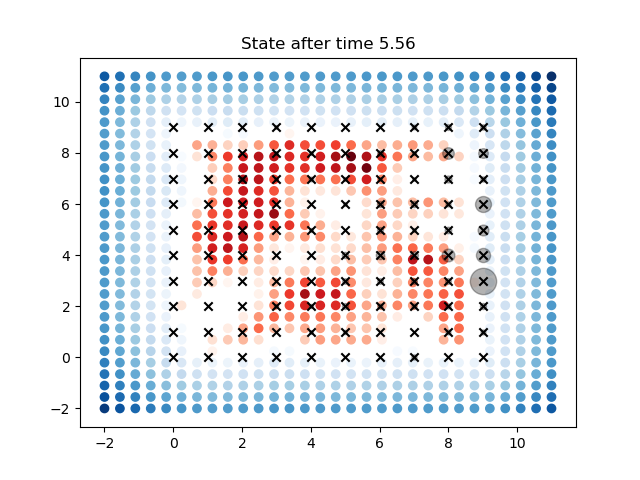
\includegraphics[width=.45\linewidth]{figures/mu_dis_edge/img02.png} }}%

\subfloat{{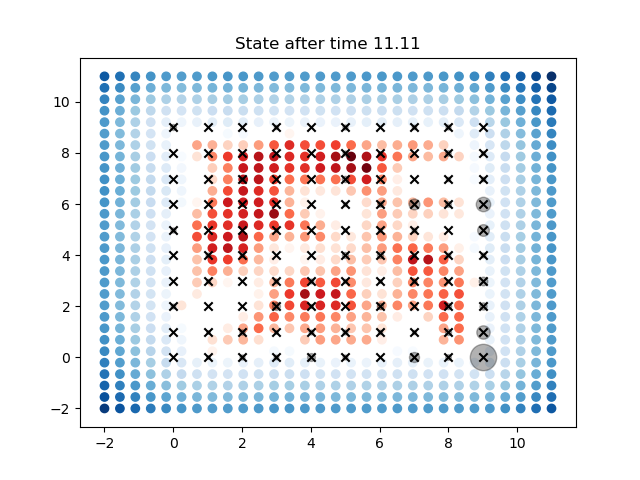
\includegraphics[width =.45\linewidth]{figures/mu_dis_edge/img03.png} }}%
\subfloat{{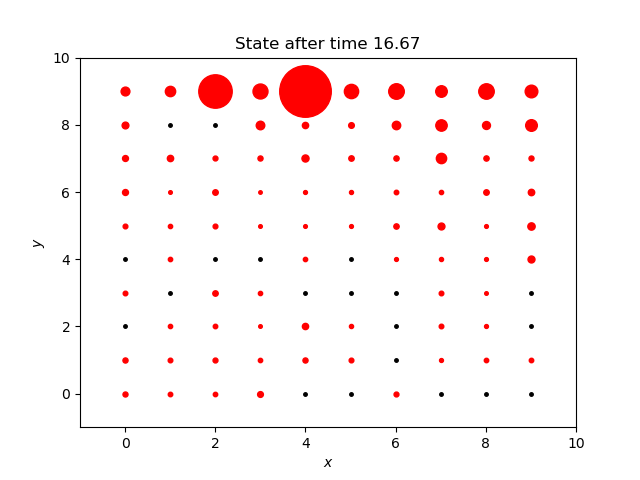
\includegraphics[width =.45\linewidth]{figures/mu_dis_edge/img04.png} }}%

\subfloat{{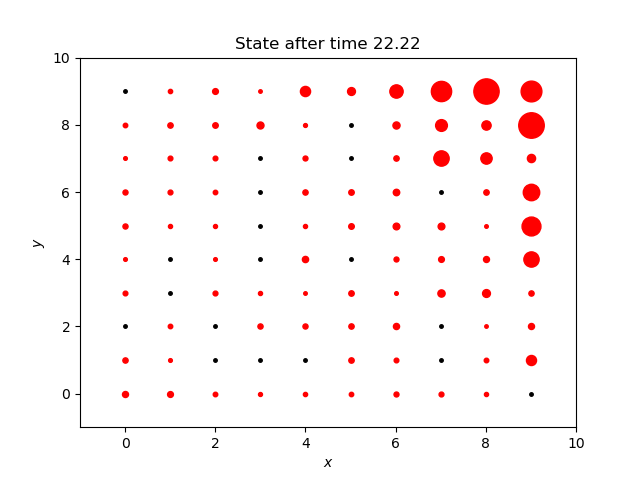
\includegraphics[width=.45\linewidth]{figures/mu_dis_edge/img05.png} }}%
\subfloat{{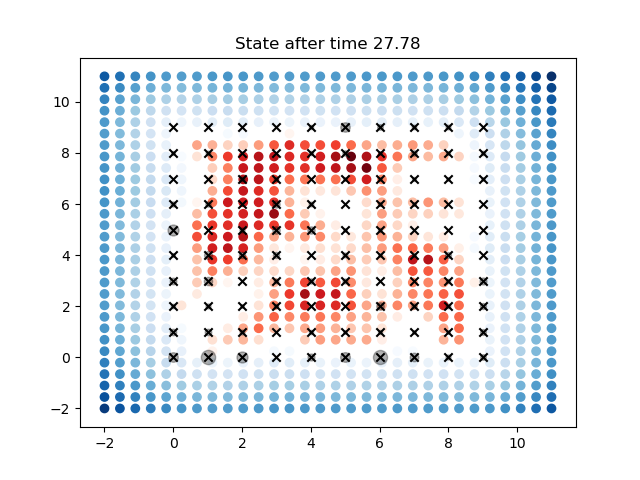
\includegraphics[width=.45\linewidth]{figures/mu_dis_edge/img06.png} }}%

\subfloat{{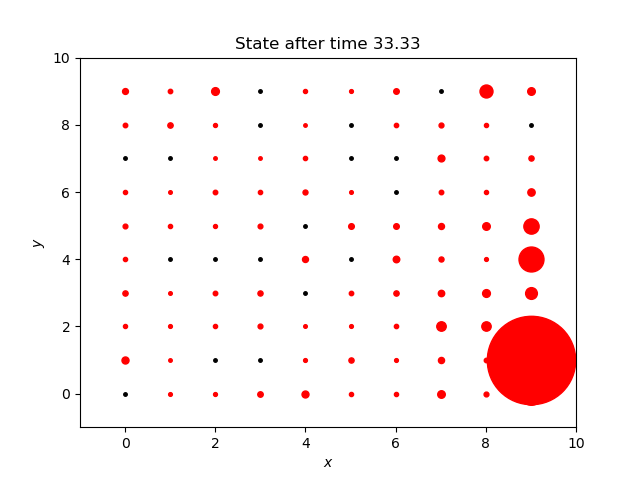
\includegraphics[width =.45\linewidth]{figures/mu_dis_edge/img07.png} }}%
\subfloat{{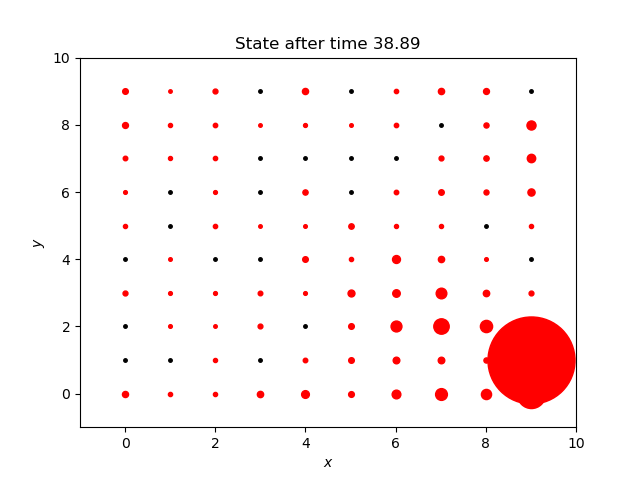
\includegraphics[width =.45\linewidth]{figures/mu_dis_edge/img08.png} }}%
\caption{Propagation on Edge of $p_x + ip_y$ Model with Onsite Disorder: with parameters as in Figure \ref{fig:pxipy_prop}, we now add onsite disorder to the lattice, letting $\mu$ for each site be chosen uniformly at random on $[0.5,3.5]$.
We initialize a state on the edge of the lattice, where there is still somewhat of a boundary between the index 1 interior and index 0 exterior.
The state disperses more so than in Figures \ref{fig:pxipy_prop} and \ref{fig:pos_dis_prop}, but it still propagates along the edge.
}%
\label{fig:mu_dis_edge_prop}%
\end{figure}

\begin{figure}
\centering
\subfloat{{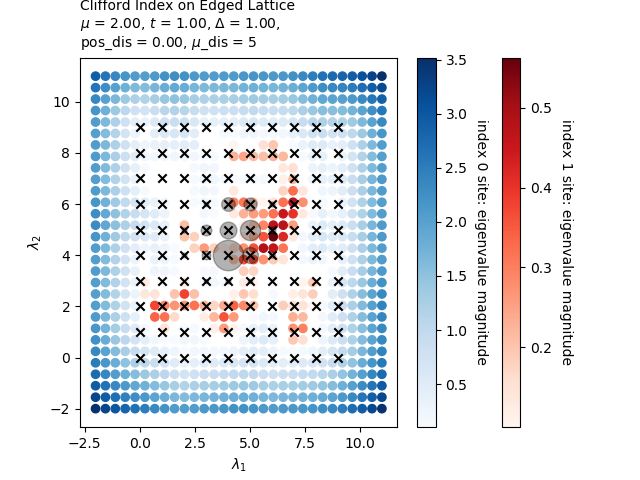
\includegraphics[width=.45\linewidth]{figures/mu_dis_interior/img01.png} }}%
\subfloat{{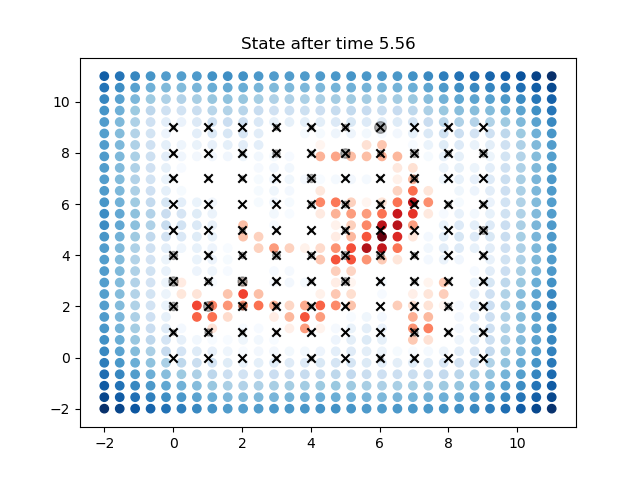
\includegraphics[width=.45\linewidth]{figures/mu_dis_interior/img02.png} }}%

\subfloat{{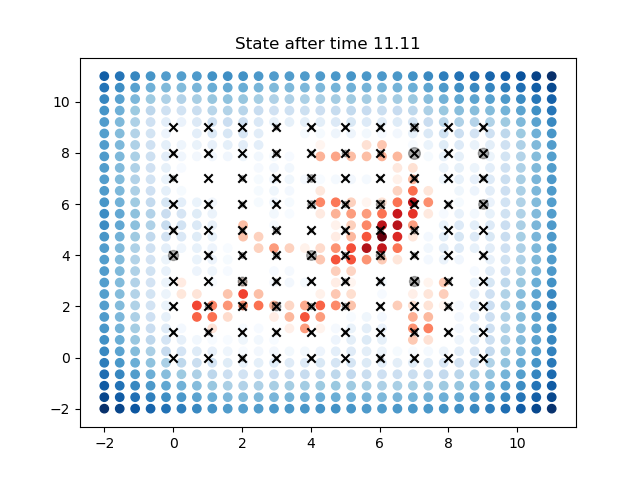
\includegraphics[width =.45\linewidth]{figures/mu_dis_interior/img03.png} }}%
\subfloat{{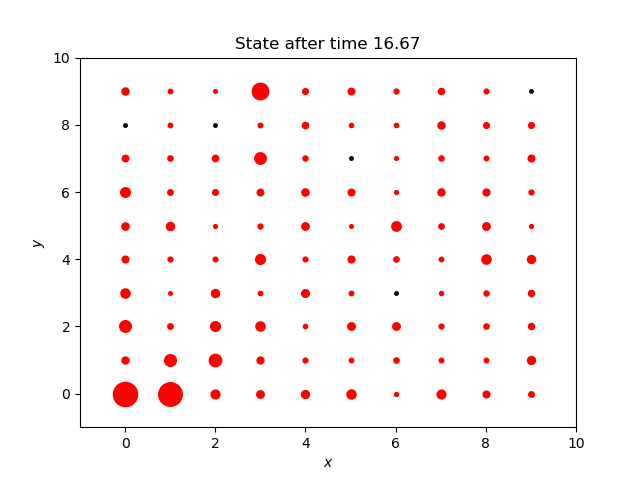
\includegraphics[width =.45\linewidth]{figures/mu_dis_interior/img04.png} }}%
\caption{Propagation on Interior of $p_x + ip_y$ Model with Onsite Disorder: with parameters as in Figure \ref{fig:pxipy_prop}, we now increase disorder, letting $\mu$ for each site be chosen uniformly at random on $[-.5,4.5]$.
We do this to obtain points of both index 1 and 0 in the interior of the lattice.
We initialize a state in the interior and hope to see propagation along the edge of the index 1 region to its right.
However the state disperses into bulk states almost immediately.
We believe this is because there is not an abrupt change of index in the interior, failing to create a coherent boundary as in Figures \ref{fig:pxipy_prop},  \ref{fig:pos_dis_prop}, and \ref{fig:mu_dis_edge_prop}.
}%
\label{fig:mu_dis_interior_prop}%
\end{figure}

\section{Future Work} \label{sec:fut}

In terms of directions for future study, we would like to understand the mechanism behind why we failed to see propagation of states around areas of nonzero Clifford index in the bulk. We expected to see such propagation, as the transition from zero to nonzero Clifford index is similar to that at the edge, so understanding where there is a difference in behavior is an interesting problem yet to be solved.

\printbibliography

\end{document}
